\documentclass[11pt]{article}
\usepackage[textwidth=18.0cm, textheight=23.0cm, top=2.0cm]{geometry}
\usepackage{pst-all}
\usepackage{amssymb}
\usepackage{tikz}
\usepackage{underscore}\begin{document}
\pagestyle{empty}


ClassName: \underline{\textbf{Class_03.2bp-40}}
\par
BinSize: \underline{\textbf{40 × 40}}
\par
ReduceSize: \underline{\textbf{40 × 40}}
\par
TypeNum: \underline{\textbf{98}}
\par
Num: \underline{\textbf{100}}
\par
OutS: \underline{\textbf{30400}}
\par
InS: \underline{\textbf{28723}}
\par
Rate: \underline{\textbf{0.945}}
\par
UB: \underline{\textbf{19}}
\par
LB0: \underline{\textbf{19}}
\par
LB: \underline{\textbf{19}}
\par
LBWithCut: \underline{\textbf{19}}
\par
NodeCut: \underline{\textbf{0}}
\par
ExtendedNodeCnt: \underline{\textbf{1}}
\par
GenNodeCnt: \underline{\textbf{1}}
\par
PrimalNode: \underline{\textbf{0}}
\par
ColumnCount: \underline{\textbf{19}}
\par
TotalCutCount: \underline{\textbf{0}}
\par
RootCutCount: \underline{\textbf{0}}
\par
LPSolverCnt: \underline{\textbf{1}}
\par
PricingSolverCnt: \underline{\textbf{0}}
\par
BranchAndBoundNum: \underline{\textbf{1}}
\par
isOpt: \underline{\textbf{true}}
\par
TimeOnInitSolution: \underline{\textbf{600.000 s}}
\par
TimeOnPrimal: \underline{\textbf{0.000 s}}
\par
TimeOnPricing: \underline{\textbf{0.000 s}}
\par
TimeOnRmp: \underline{\textbf{0.062 s}}
\par
TotalTime: \underline{\textbf{600.375 s}}
\par
\newpage


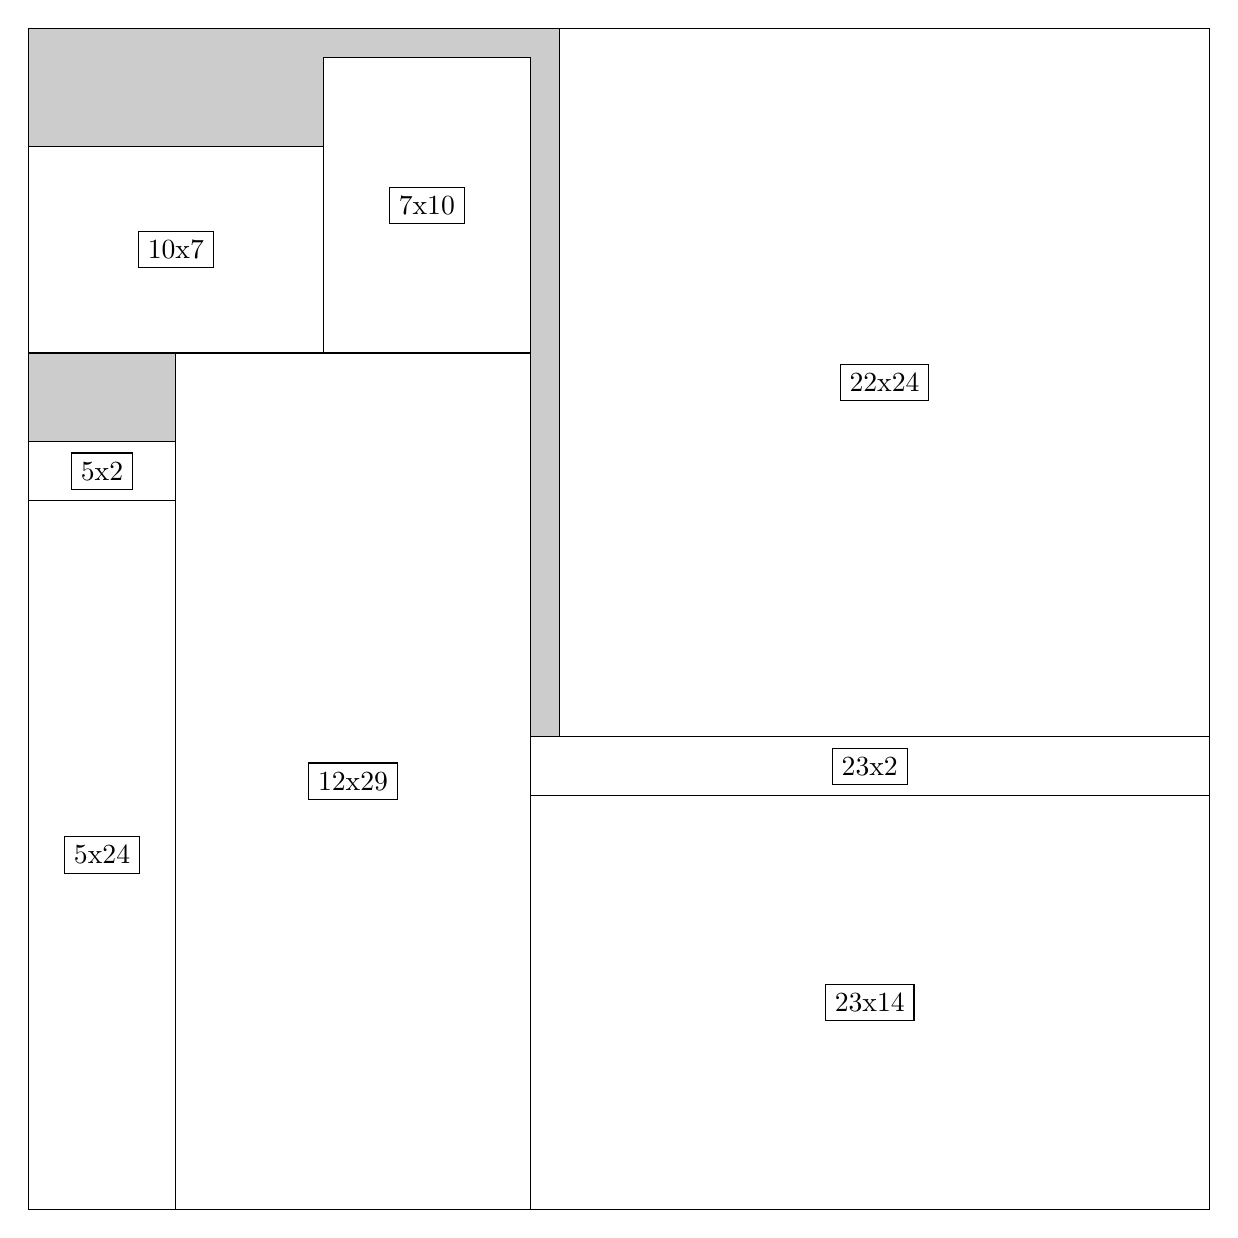
\begin{tikzpicture}[shorten >=1pt,scale=1.0,every node/.style={scale=1.0},->]
\tikzstyle{vertex}=[circle,fill=black!25,minimum size=14pt,inner sep=0pt]
\filldraw[fill=gray!40!white, draw=black] (0,0) rectangle (15.0,15.0);
\foreach \name/\x/\y/\w/\h in {23x14/6.375/0.0/8.625/5.25,23x2/6.375/5.25/8.625/0.75,22x24/6.75/6.0/8.25/9.0,12x29/1.875/0.0/4.5/10.875,5x24/0.0/0.0/1.875/9.0,5x2/0.0/9.0/1.875/0.75,7x10/3.75/10.875/2.625/3.75,10x7/0.0/10.875/3.75/2.625}
\filldraw[fill=white!40!white, draw=black] (\x,\y) rectangle node[draw] (\name) {\name} ++(\w,\h);
\end{tikzpicture}


w =23 , h =14 , x =17 , y =0 , v =322
\par
w =23 , h =2 , x =17 , y =14 , v =46
\par
w =22 , h =24 , x =18 , y =16 , v =528
\par
w =12 , h =29 , x =5 , y =0 , v =348
\par
w =5 , h =24 , x =0 , y =0 , v =120
\par
w =5 , h =2 , x =0 , y =24 , v =10
\par
w =7 , h =10 , x =10 , y =29 , v =70
\par
w =10 , h =7 , x =0 , y =29 , v =70
\par
\newpage


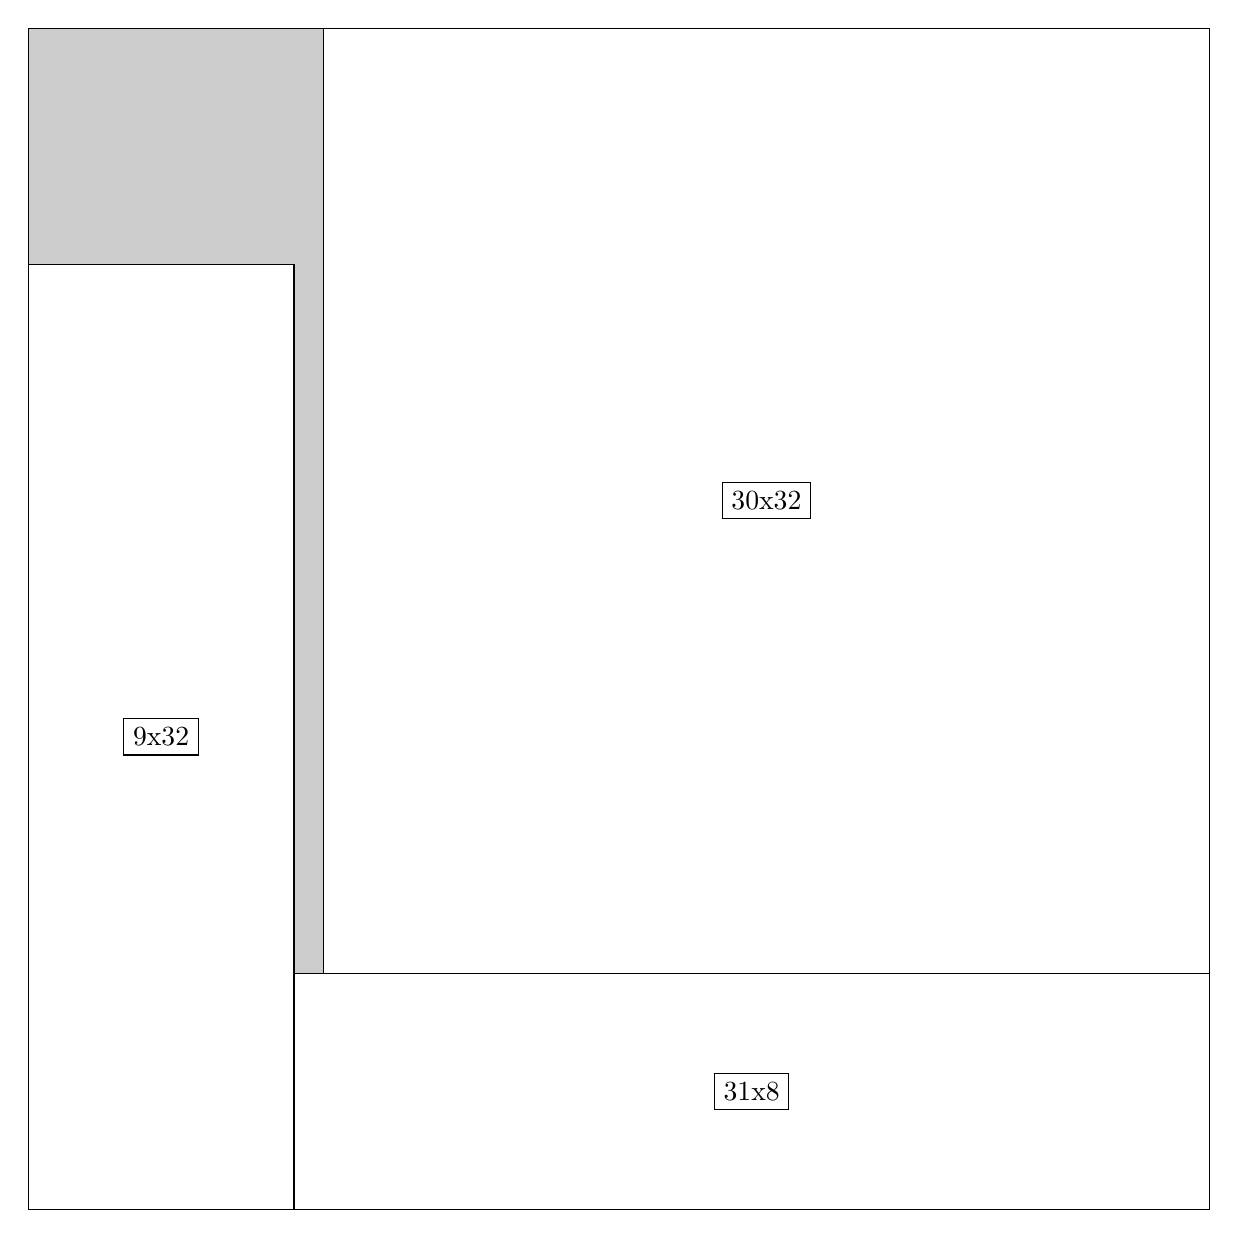
\begin{tikzpicture}[shorten >=1pt,scale=1.0,every node/.style={scale=1.0},->]
\tikzstyle{vertex}=[circle,fill=black!25,minimum size=14pt,inner sep=0pt]
\filldraw[fill=gray!40!white, draw=black] (0,0) rectangle (15.0,15.0);
\foreach \name/\x/\y/\w/\h in {31x8/3.375/0.0/11.625/3.0,30x32/3.75/3.0/11.25/12.0,9x32/0.0/0.0/3.375/12.0}
\filldraw[fill=white!40!white, draw=black] (\x,\y) rectangle node[draw] (\name) {\name} ++(\w,\h);
\end{tikzpicture}


w =31 , h =8 , x =9 , y =0 , v =248
\par
w =30 , h =32 , x =10 , y =8 , v =960
\par
w =9 , h =32 , x =0 , y =0 , v =288
\par
\newpage


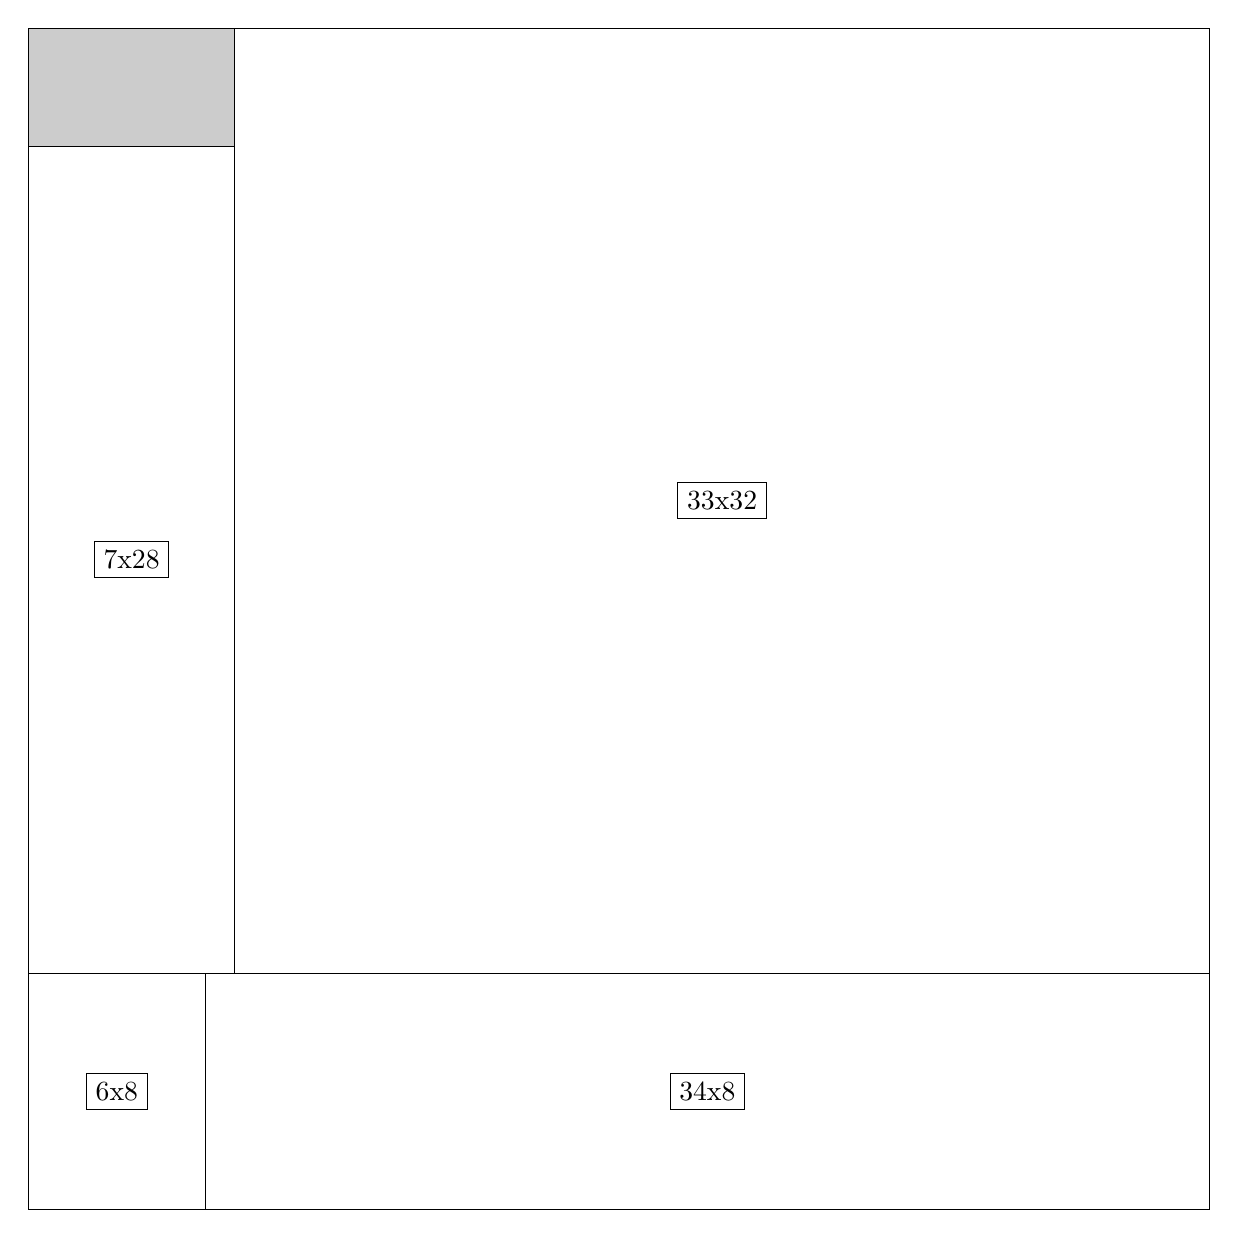
\begin{tikzpicture}[shorten >=1pt,scale=1.0,every node/.style={scale=1.0},->]
\tikzstyle{vertex}=[circle,fill=black!25,minimum size=14pt,inner sep=0pt]
\filldraw[fill=gray!40!white, draw=black] (0,0) rectangle (15.0,15.0);
\foreach \name/\x/\y/\w/\h in {34x8/2.25/0.0/12.75/3.0,6x8/0.0/0.0/2.25/3.0,33x32/2.625/3.0/12.375/12.0,7x28/0.0/3.0/2.625/10.5}
\filldraw[fill=white!40!white, draw=black] (\x,\y) rectangle node[draw] (\name) {\name} ++(\w,\h);
\end{tikzpicture}


w =34 , h =8 , x =6 , y =0 , v =272
\par
w =6 , h =8 , x =0 , y =0 , v =48
\par
w =33 , h =32 , x =7 , y =8 , v =1056
\par
w =7 , h =28 , x =0 , y =8 , v =196
\par
\newpage


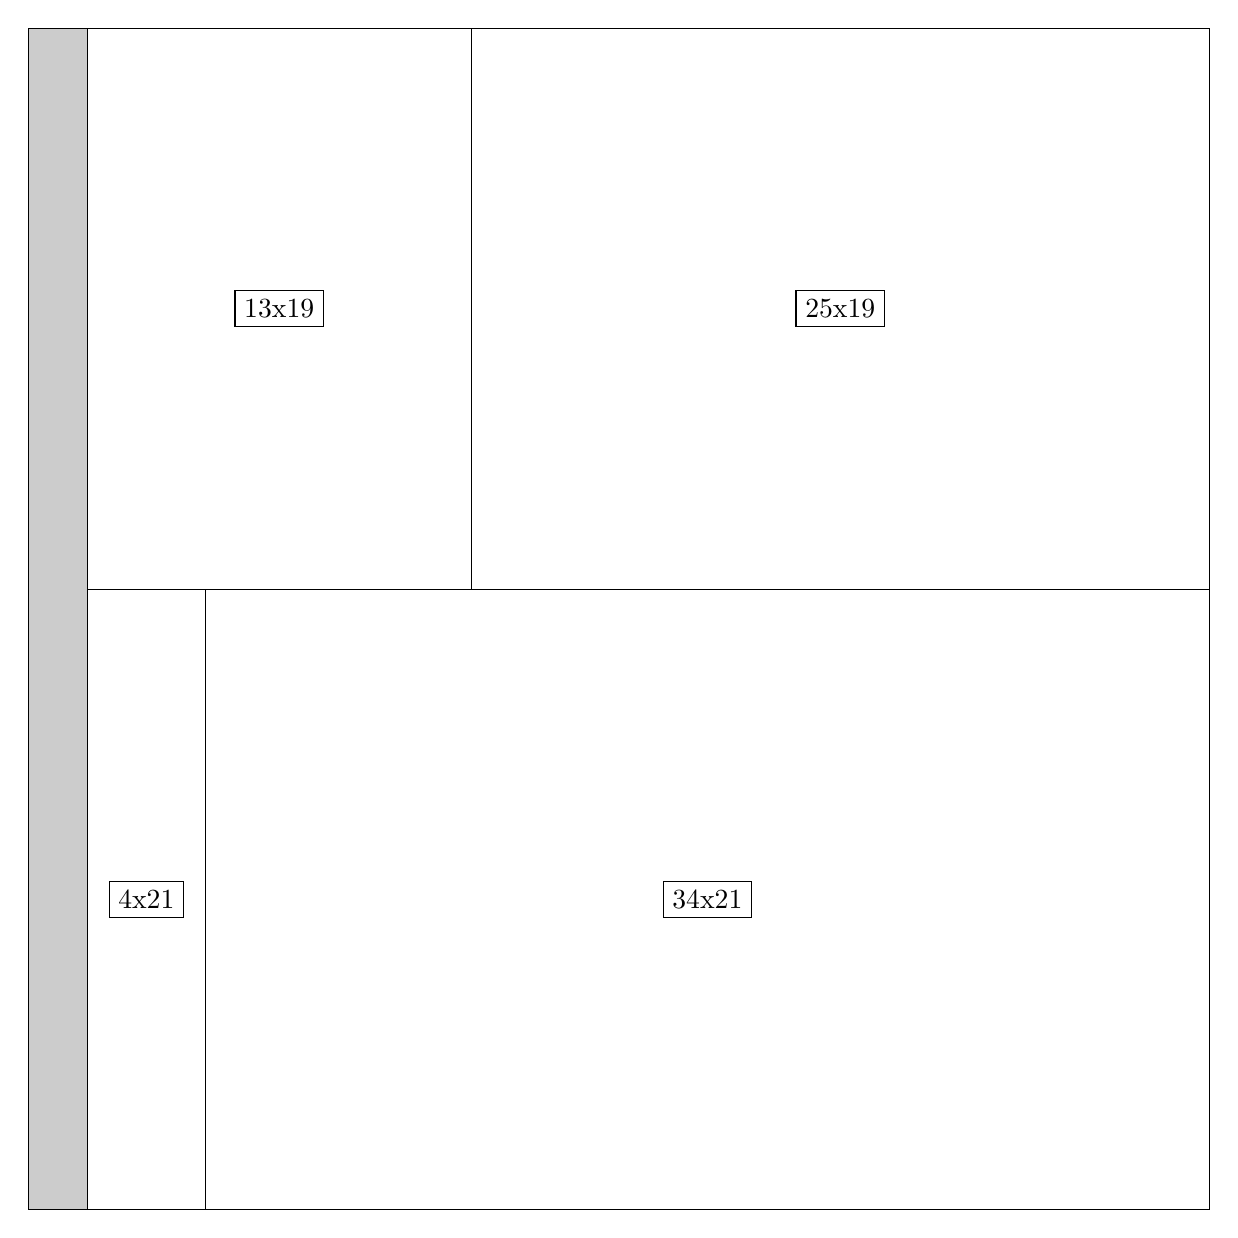
\begin{tikzpicture}[shorten >=1pt,scale=1.0,every node/.style={scale=1.0},->]
\tikzstyle{vertex}=[circle,fill=black!25,minimum size=14pt,inner sep=0pt]
\filldraw[fill=gray!40!white, draw=black] (0,0) rectangle (15.0,15.0);
\foreach \name/\x/\y/\w/\h in {34x21/2.25/0.0/12.75/7.875,4x21/0.75/0.0/1.5/7.875,25x19/5.625/7.875/9.375/7.125,13x19/0.75/7.875/4.875/7.125}
\filldraw[fill=white!40!white, draw=black] (\x,\y) rectangle node[draw] (\name) {\name} ++(\w,\h);
\end{tikzpicture}


w =34 , h =21 , x =6 , y =0 , v =714
\par
w =4 , h =21 , x =2 , y =0 , v =84
\par
w =25 , h =19 , x =15 , y =21 , v =475
\par
w =13 , h =19 , x =2 , y =21 , v =247
\par
\newpage


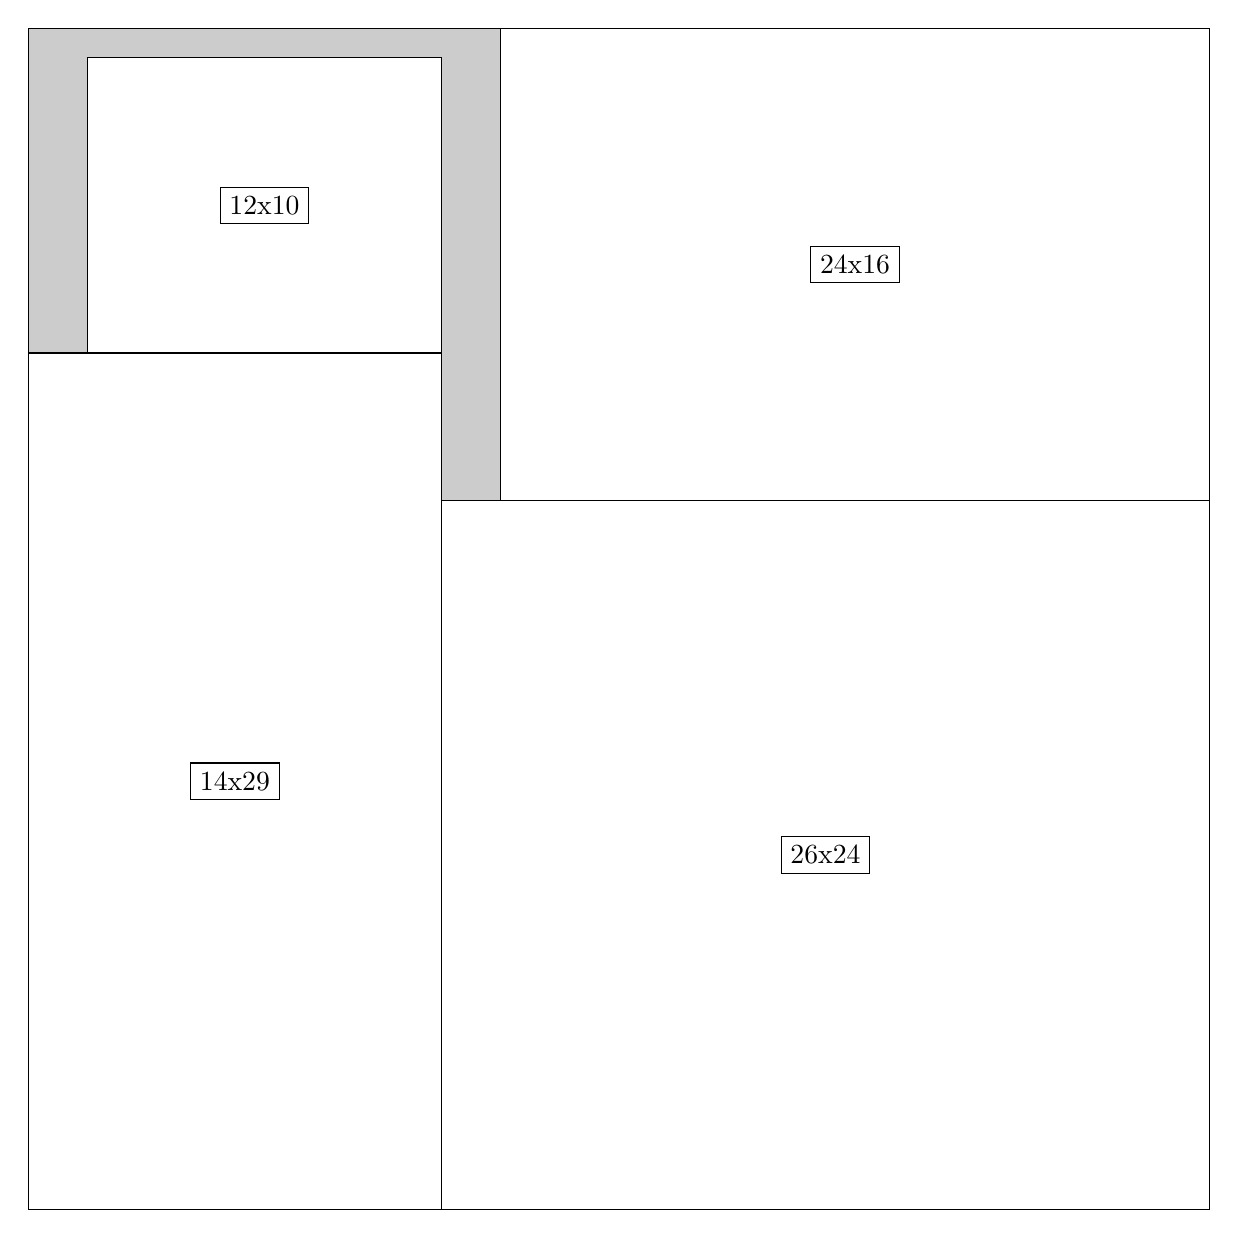
\begin{tikzpicture}[shorten >=1pt,scale=1.0,every node/.style={scale=1.0},->]
\tikzstyle{vertex}=[circle,fill=black!25,minimum size=14pt,inner sep=0pt]
\filldraw[fill=gray!40!white, draw=black] (0,0) rectangle (15.0,15.0);
\foreach \name/\x/\y/\w/\h in {26x24/5.25/0.0/9.75/9.0,24x16/6.0/9.0/9.0/6.0,14x29/0.0/0.0/5.25/10.875,12x10/0.75/10.875/4.5/3.75}
\filldraw[fill=white!40!white, draw=black] (\x,\y) rectangle node[draw] (\name) {\name} ++(\w,\h);
\end{tikzpicture}


w =26 , h =24 , x =14 , y =0 , v =624
\par
w =24 , h =16 , x =16 , y =24 , v =384
\par
w =14 , h =29 , x =0 , y =0 , v =406
\par
w =12 , h =10 , x =2 , y =29 , v =120
\par
\newpage


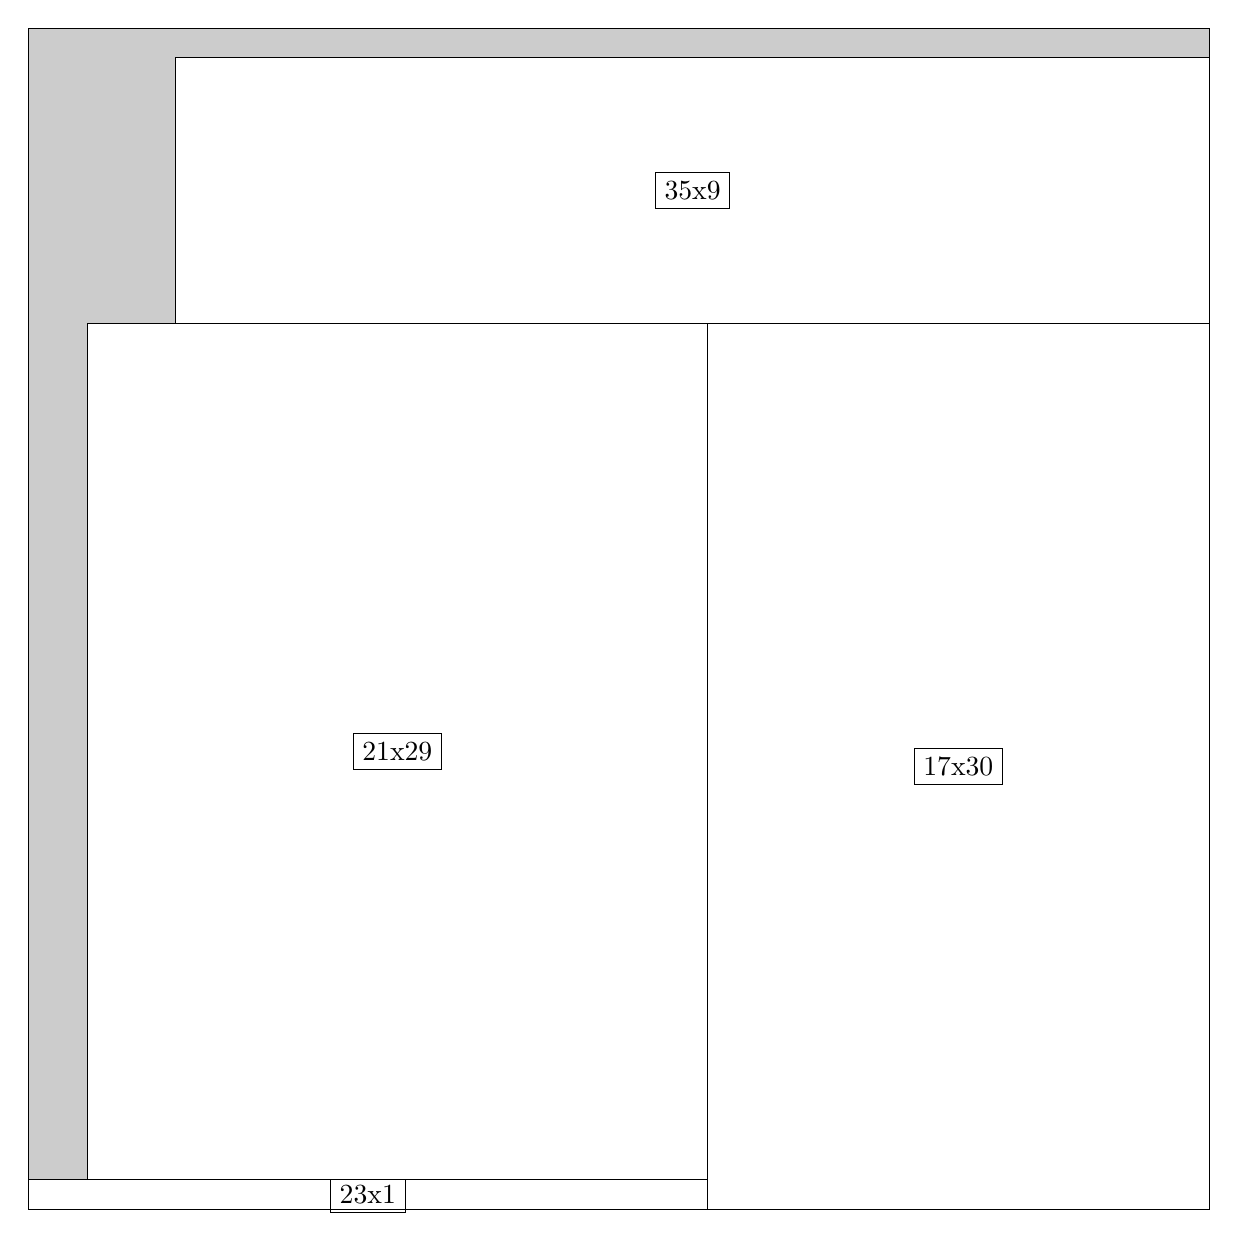
\begin{tikzpicture}[shorten >=1pt,scale=1.0,every node/.style={scale=1.0},->]
\tikzstyle{vertex}=[circle,fill=black!25,minimum size=14pt,inner sep=0pt]
\filldraw[fill=gray!40!white, draw=black] (0,0) rectangle (15.0,15.0);
\foreach \name/\x/\y/\w/\h in {17x30/8.625/0.0/6.375/11.25,23x1/0.0/0.0/8.625/0.375,21x29/0.75/0.375/7.875/10.875,35x9/1.875/11.25/13.125/3.375}
\filldraw[fill=white!40!white, draw=black] (\x,\y) rectangle node[draw] (\name) {\name} ++(\w,\h);
\end{tikzpicture}


w =17 , h =30 , x =23 , y =0 , v =510
\par
w =23 , h =1 , x =0 , y =0 , v =23
\par
w =21 , h =29 , x =2 , y =1 , v =609
\par
w =35 , h =9 , x =5 , y =30 , v =315
\par
\newpage


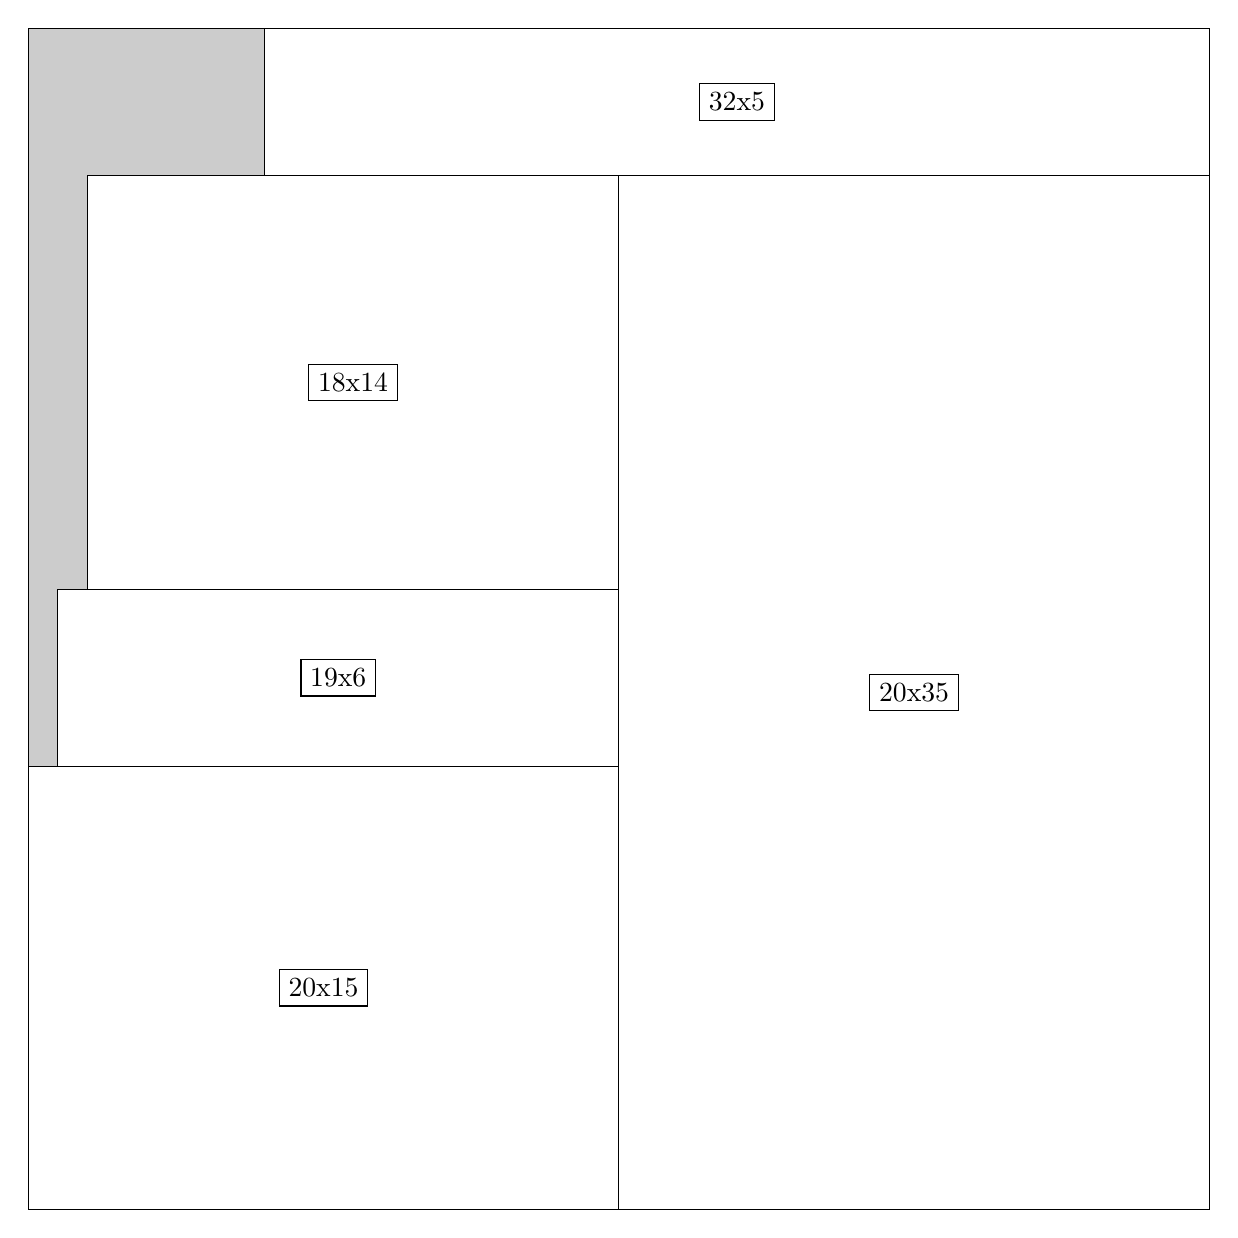
\begin{tikzpicture}[shorten >=1pt,scale=1.0,every node/.style={scale=1.0},->]
\tikzstyle{vertex}=[circle,fill=black!25,minimum size=14pt,inner sep=0pt]
\filldraw[fill=gray!40!white, draw=black] (0,0) rectangle (15.0,15.0);
\foreach \name/\x/\y/\w/\h in {20x35/7.5/0.0/7.5/13.125,20x15/0.0/0.0/7.5/5.625,19x6/0.375/5.625/7.125/2.25,18x14/0.75/7.875/6.75/5.25,32x5/3.0/13.125/12.0/1.875}
\filldraw[fill=white!40!white, draw=black] (\x,\y) rectangle node[draw] (\name) {\name} ++(\w,\h);
\end{tikzpicture}


w =20 , h =35 , x =20 , y =0 , v =700
\par
w =20 , h =15 , x =0 , y =0 , v =300
\par
w =19 , h =6 , x =1 , y =15 , v =114
\par
w =18 , h =14 , x =2 , y =21 , v =252
\par
w =32 , h =5 , x =8 , y =35 , v =160
\par
\newpage


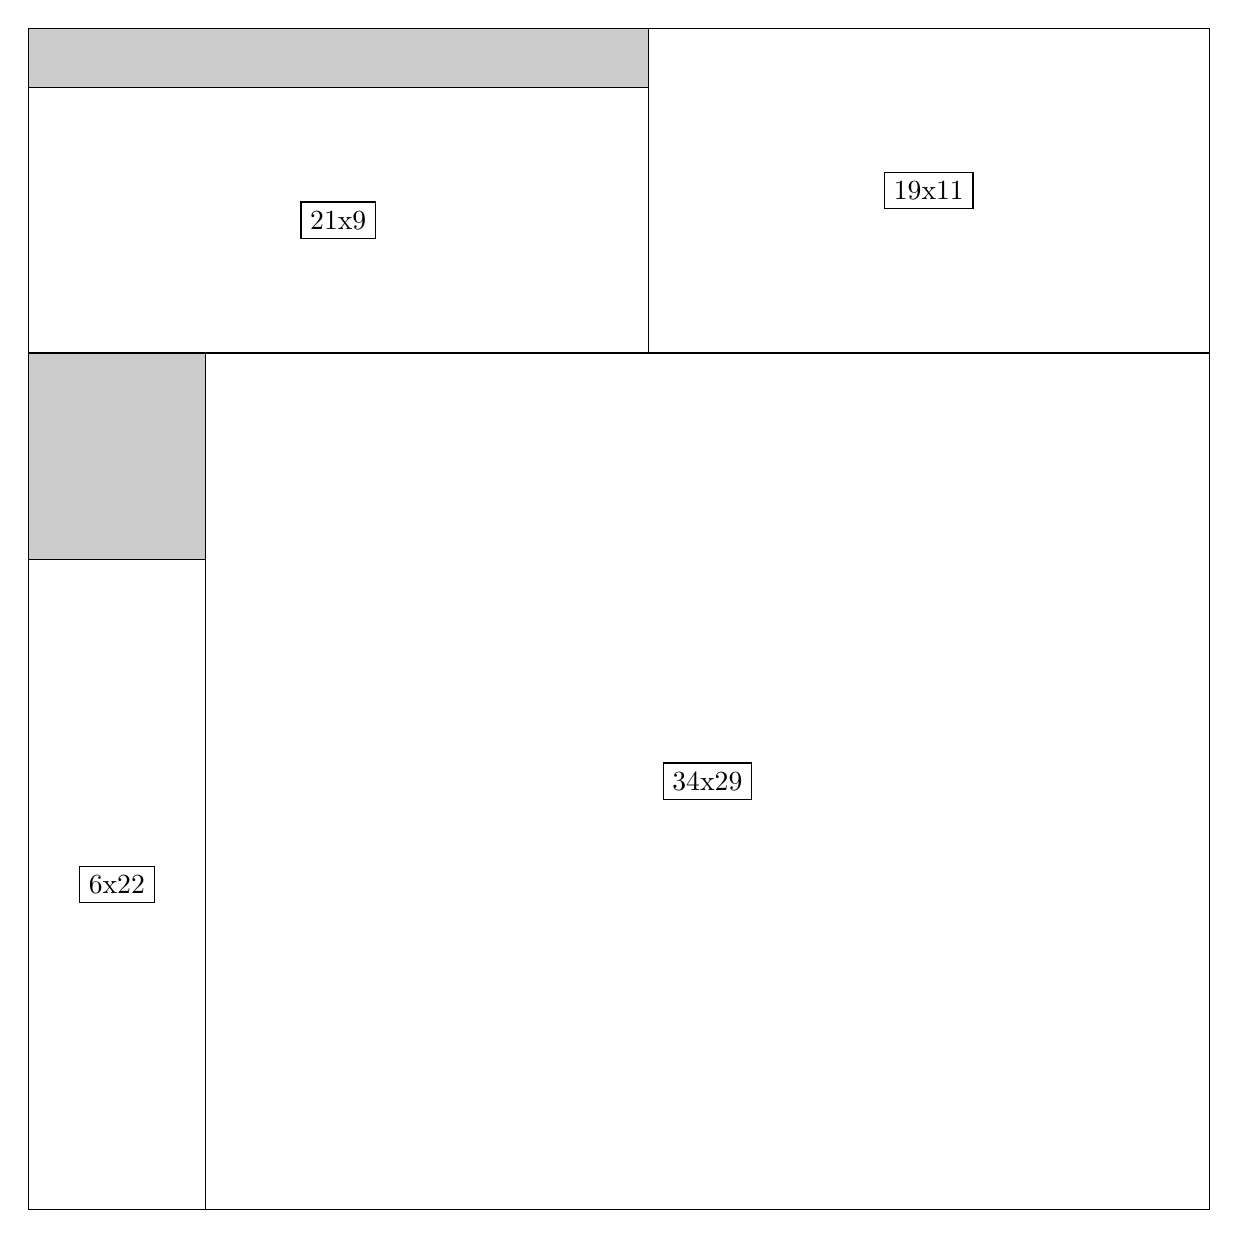
\begin{tikzpicture}[shorten >=1pt,scale=1.0,every node/.style={scale=1.0},->]
\tikzstyle{vertex}=[circle,fill=black!25,minimum size=14pt,inner sep=0pt]
\filldraw[fill=gray!40!white, draw=black] (0,0) rectangle (15.0,15.0);
\foreach \name/\x/\y/\w/\h in {34x29/2.25/0.0/12.75/10.875,6x22/0.0/0.0/2.25/8.25,19x11/7.875/10.875/7.125/4.125,21x9/0.0/10.875/7.875/3.375}
\filldraw[fill=white!40!white, draw=black] (\x,\y) rectangle node[draw] (\name) {\name} ++(\w,\h);
\end{tikzpicture}


w =34 , h =29 , x =6 , y =0 , v =986
\par
w =6 , h =22 , x =0 , y =0 , v =132
\par
w =19 , h =11 , x =21 , y =29 , v =209
\par
w =21 , h =9 , x =0 , y =29 , v =189
\par
\newpage


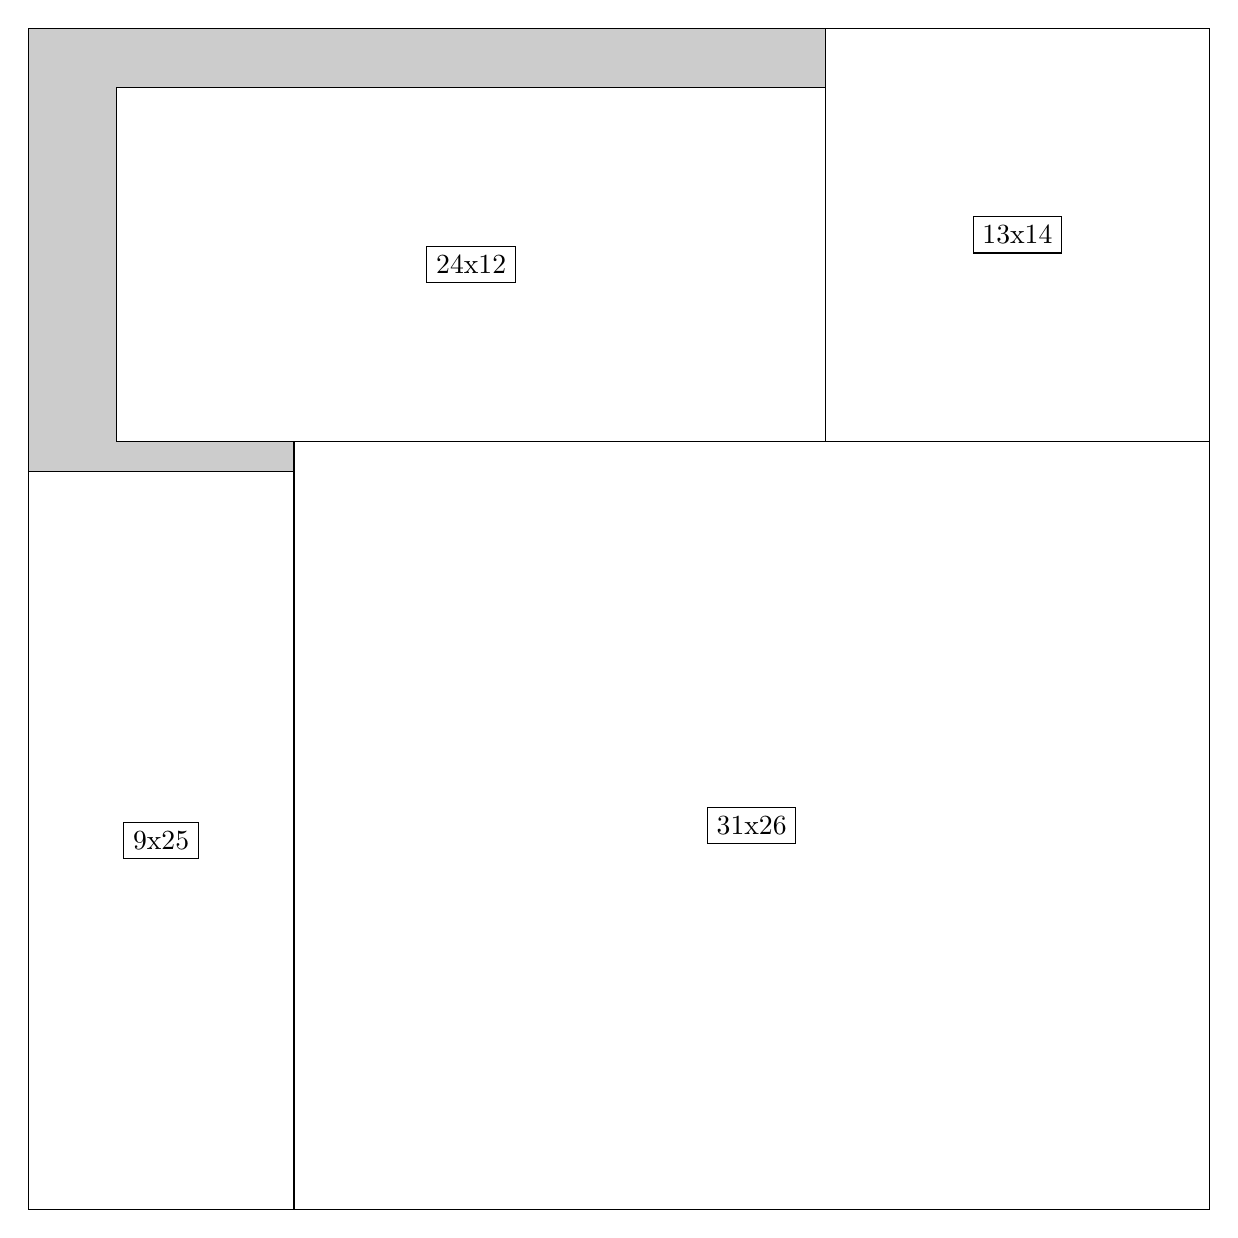
\begin{tikzpicture}[shorten >=1pt,scale=1.0,every node/.style={scale=1.0},->]
\tikzstyle{vertex}=[circle,fill=black!25,minimum size=14pt,inner sep=0pt]
\filldraw[fill=gray!40!white, draw=black] (0,0) rectangle (15.0,15.0);
\foreach \name/\x/\y/\w/\h in {31x26/3.375/0.0/11.625/9.75,9x25/0.0/0.0/3.375/9.375,13x14/10.125/9.75/4.875/5.25,24x12/1.125/9.75/9.0/4.5}
\filldraw[fill=white!40!white, draw=black] (\x,\y) rectangle node[draw] (\name) {\name} ++(\w,\h);
\end{tikzpicture}


w =31 , h =26 , x =9 , y =0 , v =806
\par
w =9 , h =25 , x =0 , y =0 , v =225
\par
w =13 , h =14 , x =27 , y =26 , v =182
\par
w =24 , h =12 , x =3 , y =26 , v =288
\par
\newpage


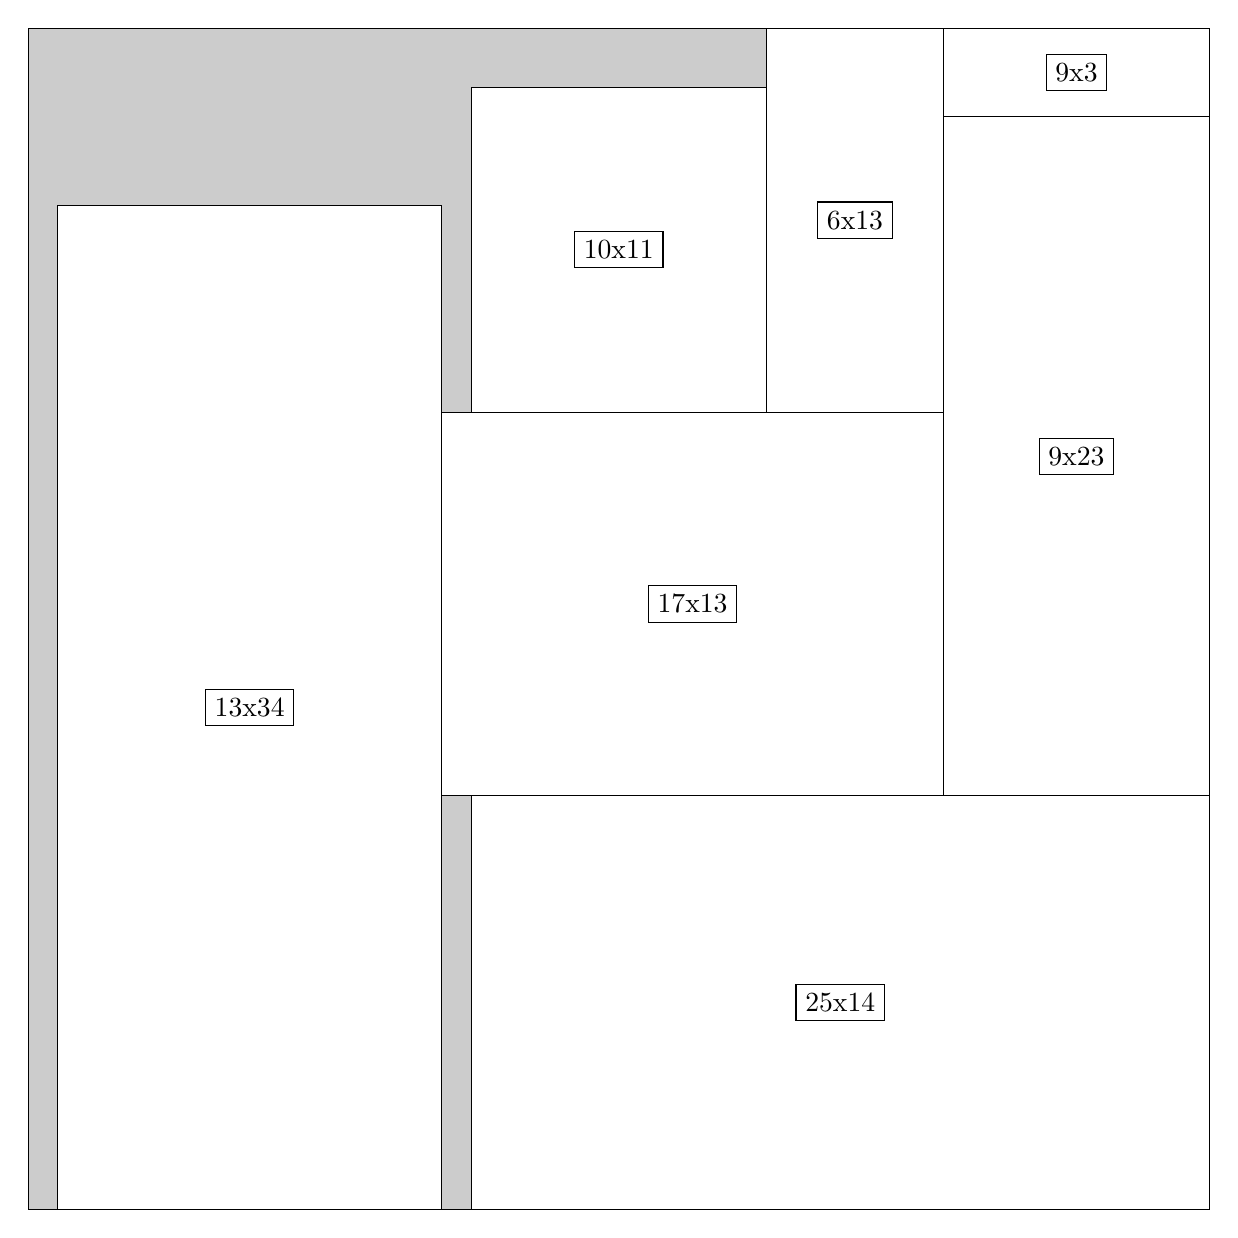
\begin{tikzpicture}[shorten >=1pt,scale=1.0,every node/.style={scale=1.0},->]
\tikzstyle{vertex}=[circle,fill=black!25,minimum size=14pt,inner sep=0pt]
\filldraw[fill=gray!40!white, draw=black] (0,0) rectangle (15.0,15.0);
\foreach \name/\x/\y/\w/\h in {25x14/5.625/0.0/9.375/5.25,9x23/11.625/5.25/3.375/8.625,9x3/11.625/13.875/3.375/1.125,17x13/5.25/5.25/6.375/4.875,6x13/9.375/10.125/2.25/4.875,10x11/5.625/10.125/3.75/4.125,13x34/0.375/0.0/4.875/12.75}
\filldraw[fill=white!40!white, draw=black] (\x,\y) rectangle node[draw] (\name) {\name} ++(\w,\h);
\end{tikzpicture}


w =25 , h =14 , x =15 , y =0 , v =350
\par
w =9 , h =23 , x =31 , y =14 , v =207
\par
w =9 , h =3 , x =31 , y =37 , v =27
\par
w =17 , h =13 , x =14 , y =14 , v =221
\par
w =6 , h =13 , x =25 , y =27 , v =78
\par
w =10 , h =11 , x =15 , y =27 , v =110
\par
w =13 , h =34 , x =1 , y =0 , v =442
\par
\newpage


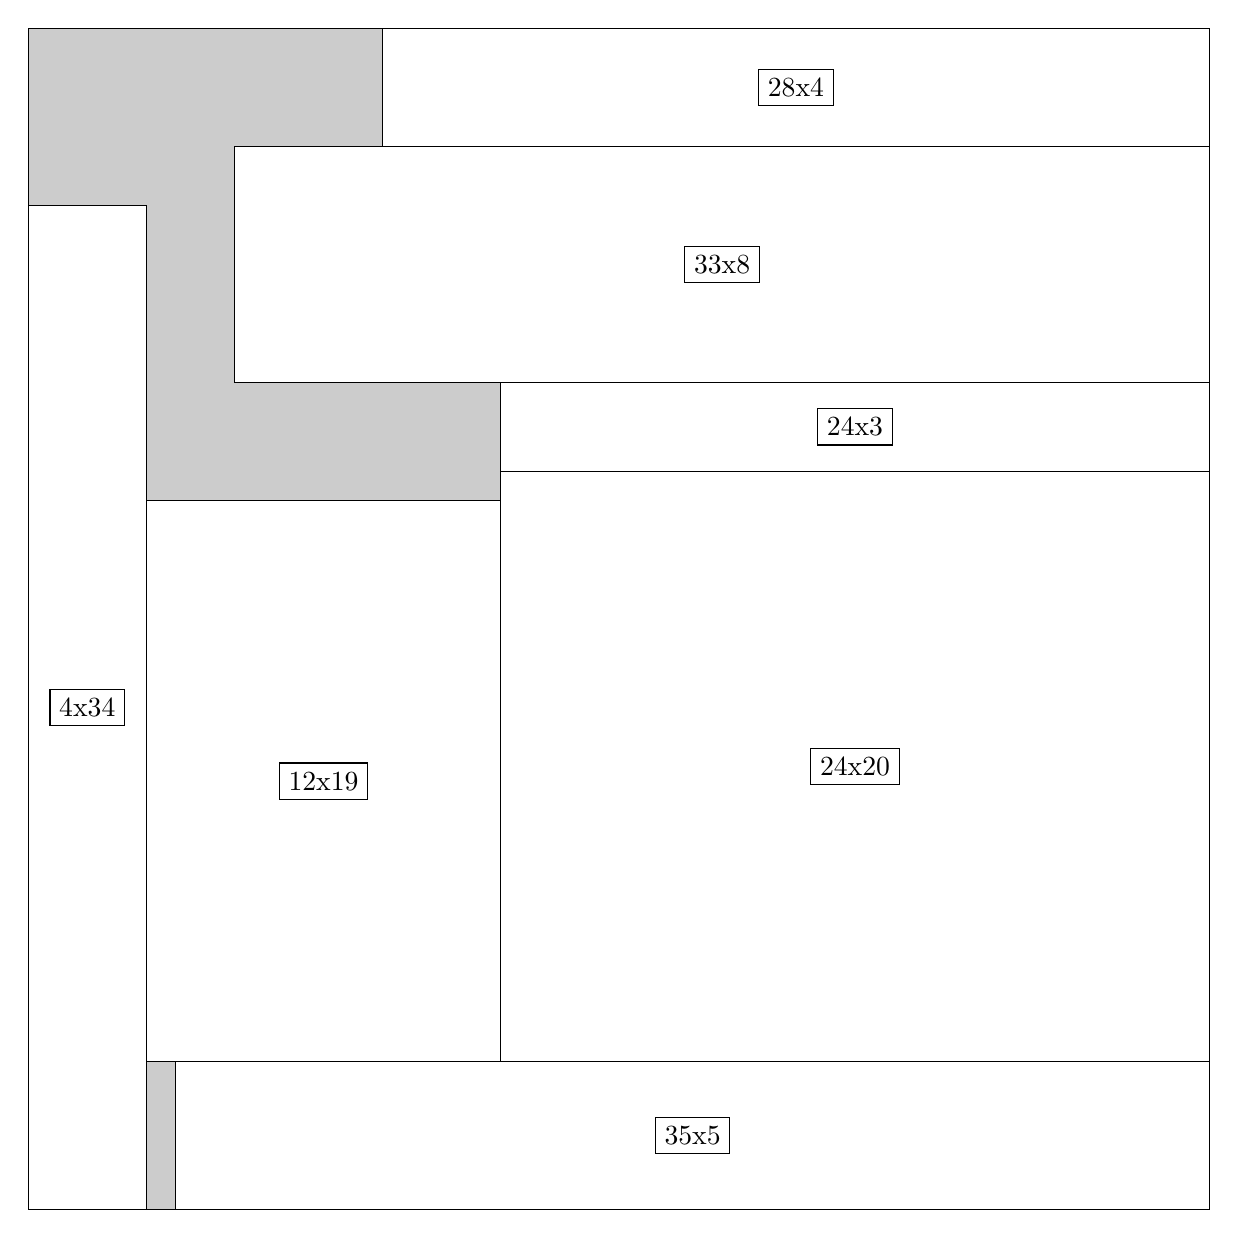
\begin{tikzpicture}[shorten >=1pt,scale=1.0,every node/.style={scale=1.0},->]
\tikzstyle{vertex}=[circle,fill=black!25,minimum size=14pt,inner sep=0pt]
\filldraw[fill=gray!40!white, draw=black] (0,0) rectangle (15.0,15.0);
\foreach \name/\x/\y/\w/\h in {35x5/1.875/0.0/13.125/1.875,24x20/6.0/1.875/9.0/7.5,24x3/6.0/9.375/9.0/1.125,12x19/1.5/1.875/4.5/7.125,33x8/2.625/10.5/12.375/3.0,28x4/4.5/13.5/10.5/1.5,4x34/0.0/0.0/1.5/12.75}
\filldraw[fill=white!40!white, draw=black] (\x,\y) rectangle node[draw] (\name) {\name} ++(\w,\h);
\end{tikzpicture}


w =35 , h =5 , x =5 , y =0 , v =175
\par
w =24 , h =20 , x =16 , y =5 , v =480
\par
w =24 , h =3 , x =16 , y =25 , v =72
\par
w =12 , h =19 , x =4 , y =5 , v =228
\par
w =33 , h =8 , x =7 , y =28 , v =264
\par
w =28 , h =4 , x =12 , y =36 , v =112
\par
w =4 , h =34 , x =0 , y =0 , v =136
\par
\newpage


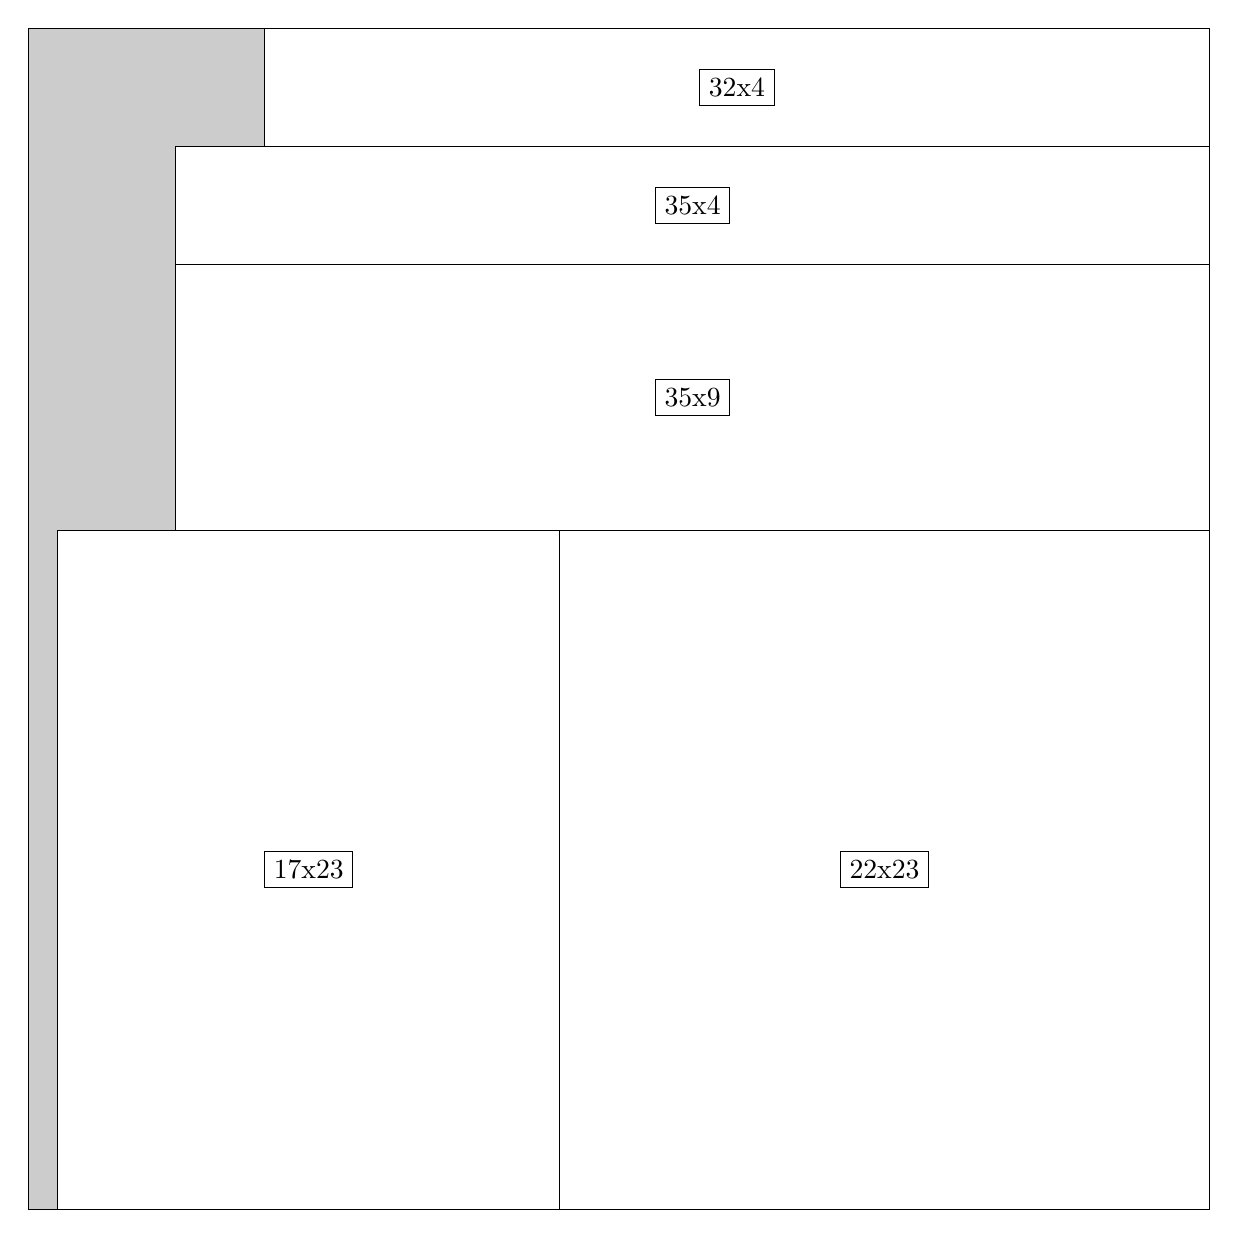
\begin{tikzpicture}[shorten >=1pt,scale=1.0,every node/.style={scale=1.0},->]
\tikzstyle{vertex}=[circle,fill=black!25,minimum size=14pt,inner sep=0pt]
\filldraw[fill=gray!40!white, draw=black] (0,0) rectangle (15.0,15.0);
\foreach \name/\x/\y/\w/\h in {22x23/6.75/0.0/8.25/8.625,17x23/0.375/0.0/6.375/8.625,35x9/1.875/8.625/13.125/3.375,35x4/1.875/12.0/13.125/1.5,32x4/3.0/13.5/12.0/1.5}
\filldraw[fill=white!40!white, draw=black] (\x,\y) rectangle node[draw] (\name) {\name} ++(\w,\h);
\end{tikzpicture}


w =22 , h =23 , x =18 , y =0 , v =506
\par
w =17 , h =23 , x =1 , y =0 , v =391
\par
w =35 , h =9 , x =5 , y =23 , v =315
\par
w =35 , h =4 , x =5 , y =32 , v =140
\par
w =32 , h =4 , x =8 , y =36 , v =128
\par
\newpage


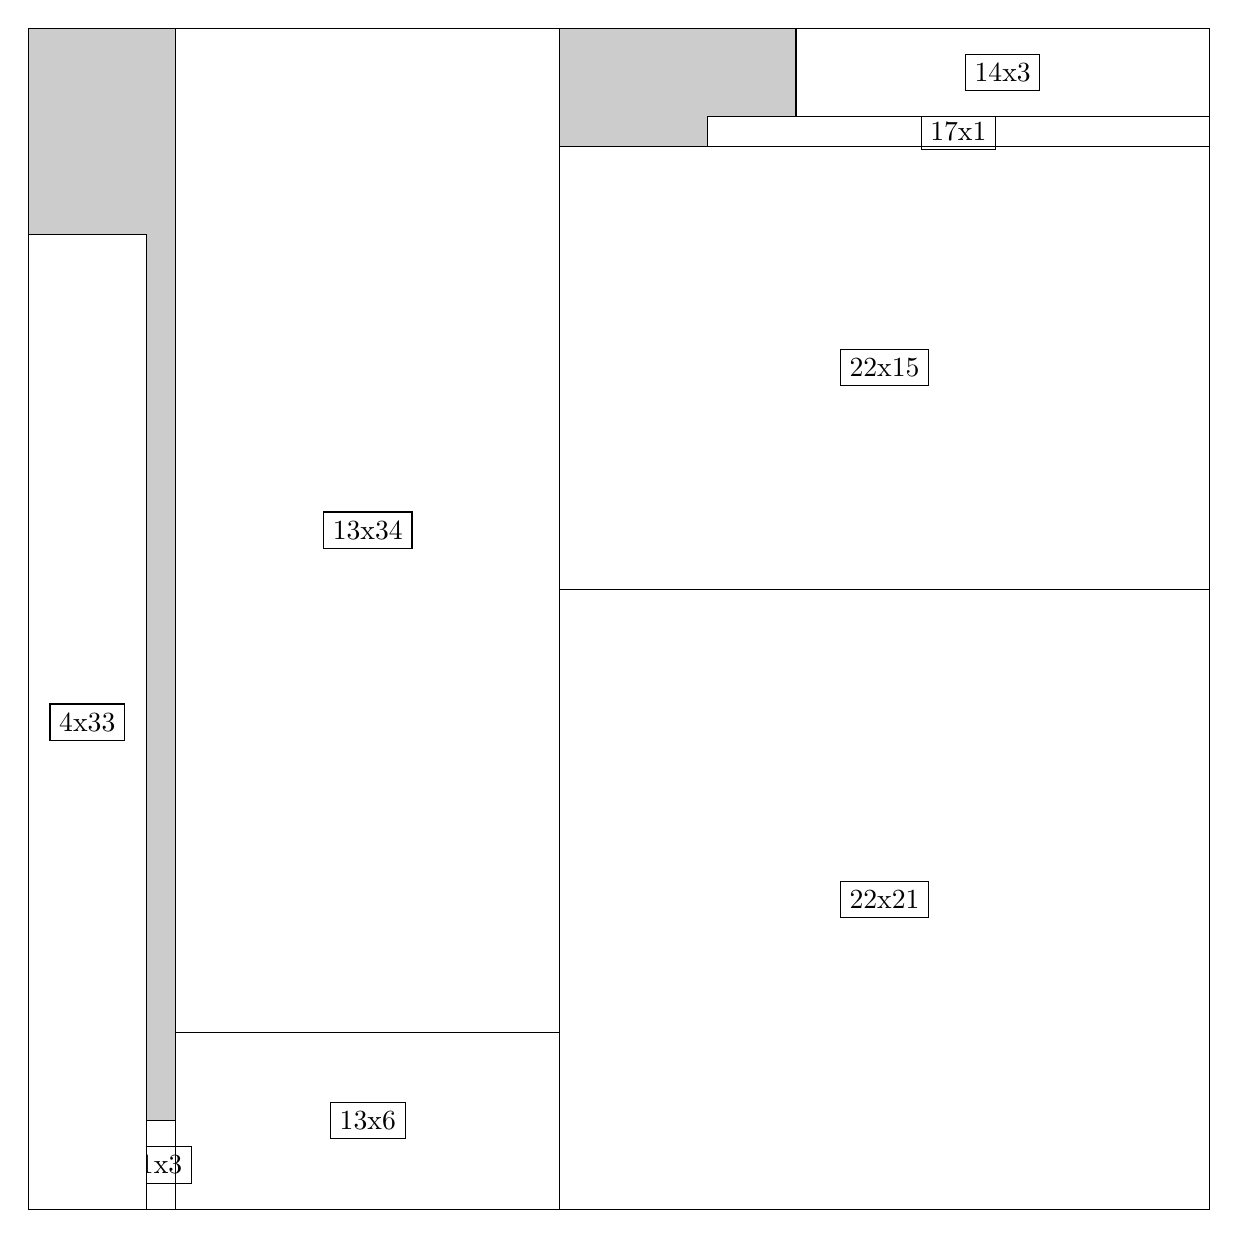
\begin{tikzpicture}[shorten >=1pt,scale=1.0,every node/.style={scale=1.0},->]
\tikzstyle{vertex}=[circle,fill=black!25,minimum size=14pt,inner sep=0pt]
\filldraw[fill=gray!40!white, draw=black] (0,0) rectangle (15.0,15.0);
\foreach \name/\x/\y/\w/\h in {22x21/6.75/0.0/8.25/7.875,22x15/6.75/7.875/8.25/5.625,17x1/8.625/13.5/6.375/0.375,14x3/9.75/13.875/5.25/1.125,13x6/1.875/0.0/4.875/2.25,1x3/1.5/0.0/0.375/1.125,13x34/1.875/2.25/4.875/12.75,4x33/0.0/0.0/1.5/12.375}
\filldraw[fill=white!40!white, draw=black] (\x,\y) rectangle node[draw] (\name) {\name} ++(\w,\h);
\end{tikzpicture}


w =22 , h =21 , x =18 , y =0 , v =462
\par
w =22 , h =15 , x =18 , y =21 , v =330
\par
w =17 , h =1 , x =23 , y =36 , v =17
\par
w =14 , h =3 , x =26 , y =37 , v =42
\par
w =13 , h =6 , x =5 , y =0 , v =78
\par
w =1 , h =3 , x =4 , y =0 , v =3
\par
w =13 , h =34 , x =5 , y =6 , v =442
\par
w =4 , h =33 , x =0 , y =0 , v =132
\par
\newpage


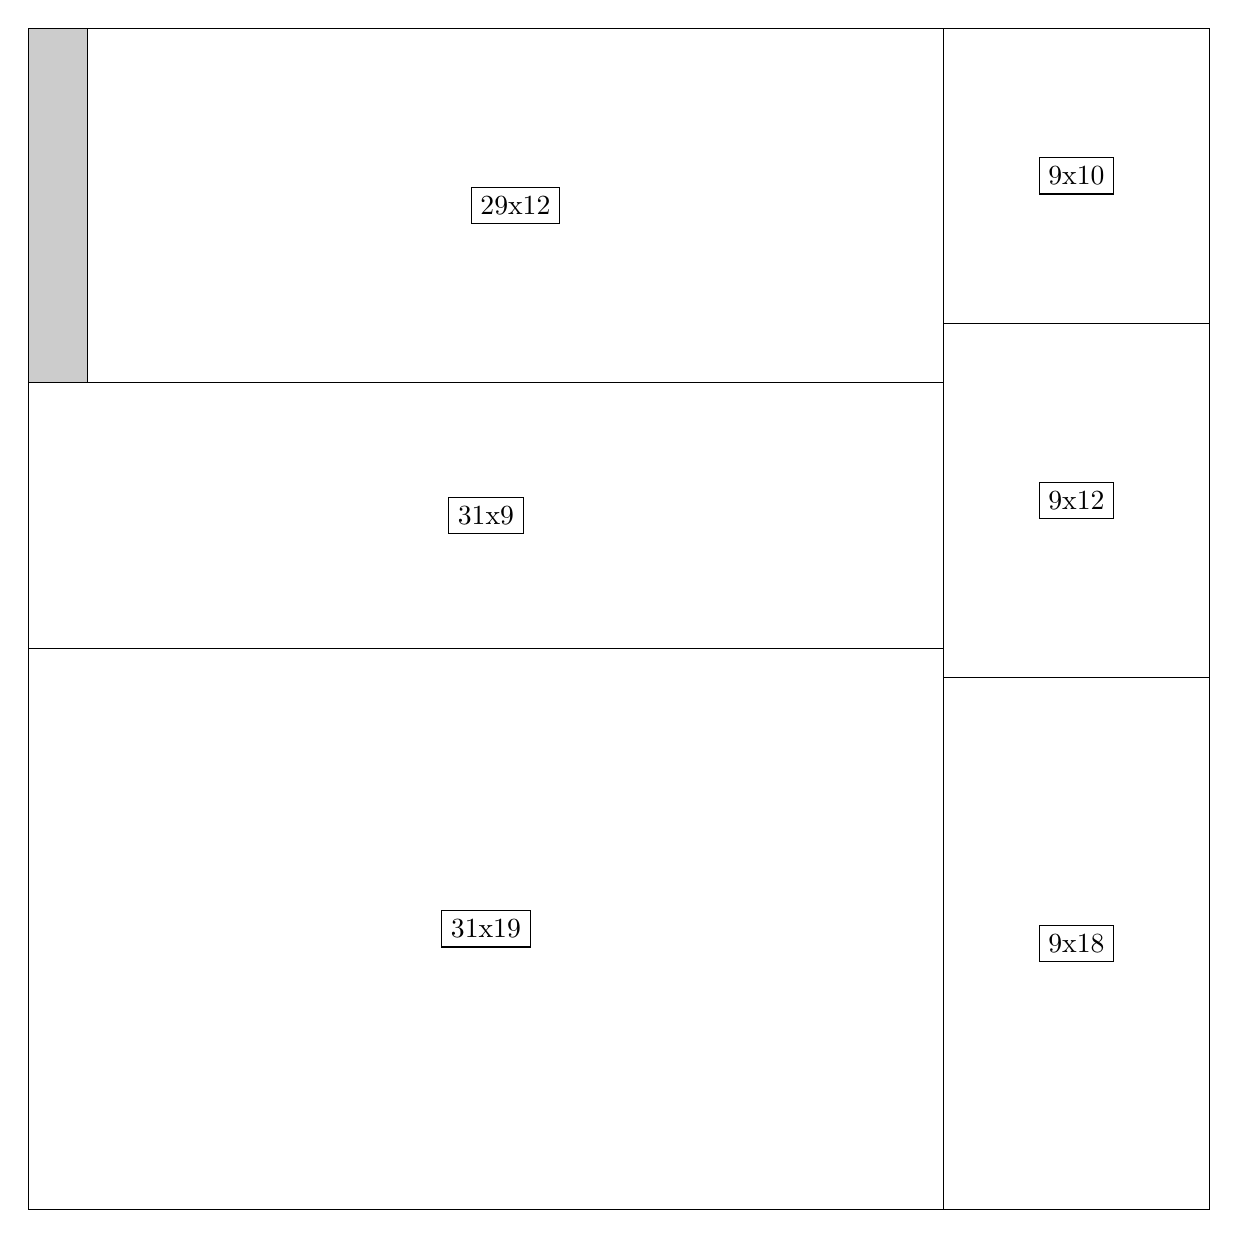
\begin{tikzpicture}[shorten >=1pt,scale=1.0,every node/.style={scale=1.0},->]
\tikzstyle{vertex}=[circle,fill=black!25,minimum size=14pt,inner sep=0pt]
\filldraw[fill=gray!40!white, draw=black] (0,0) rectangle (15.0,15.0);
\foreach \name/\x/\y/\w/\h in {9x18/11.625/0.0/3.375/6.75,9x12/11.625/6.75/3.375/4.5,9x10/11.625/11.25/3.375/3.75,31x19/0.0/0.0/11.625/7.125,31x9/0.0/7.125/11.625/3.375,29x12/0.75/10.5/10.875/4.5}
\filldraw[fill=white!40!white, draw=black] (\x,\y) rectangle node[draw] (\name) {\name} ++(\w,\h);
\end{tikzpicture}


w =9 , h =18 , x =31 , y =0 , v =162
\par
w =9 , h =12 , x =31 , y =18 , v =108
\par
w =9 , h =10 , x =31 , y =30 , v =90
\par
w =31 , h =19 , x =0 , y =0 , v =589
\par
w =31 , h =9 , x =0 , y =19 , v =279
\par
w =29 , h =12 , x =2 , y =28 , v =348
\par
\newpage


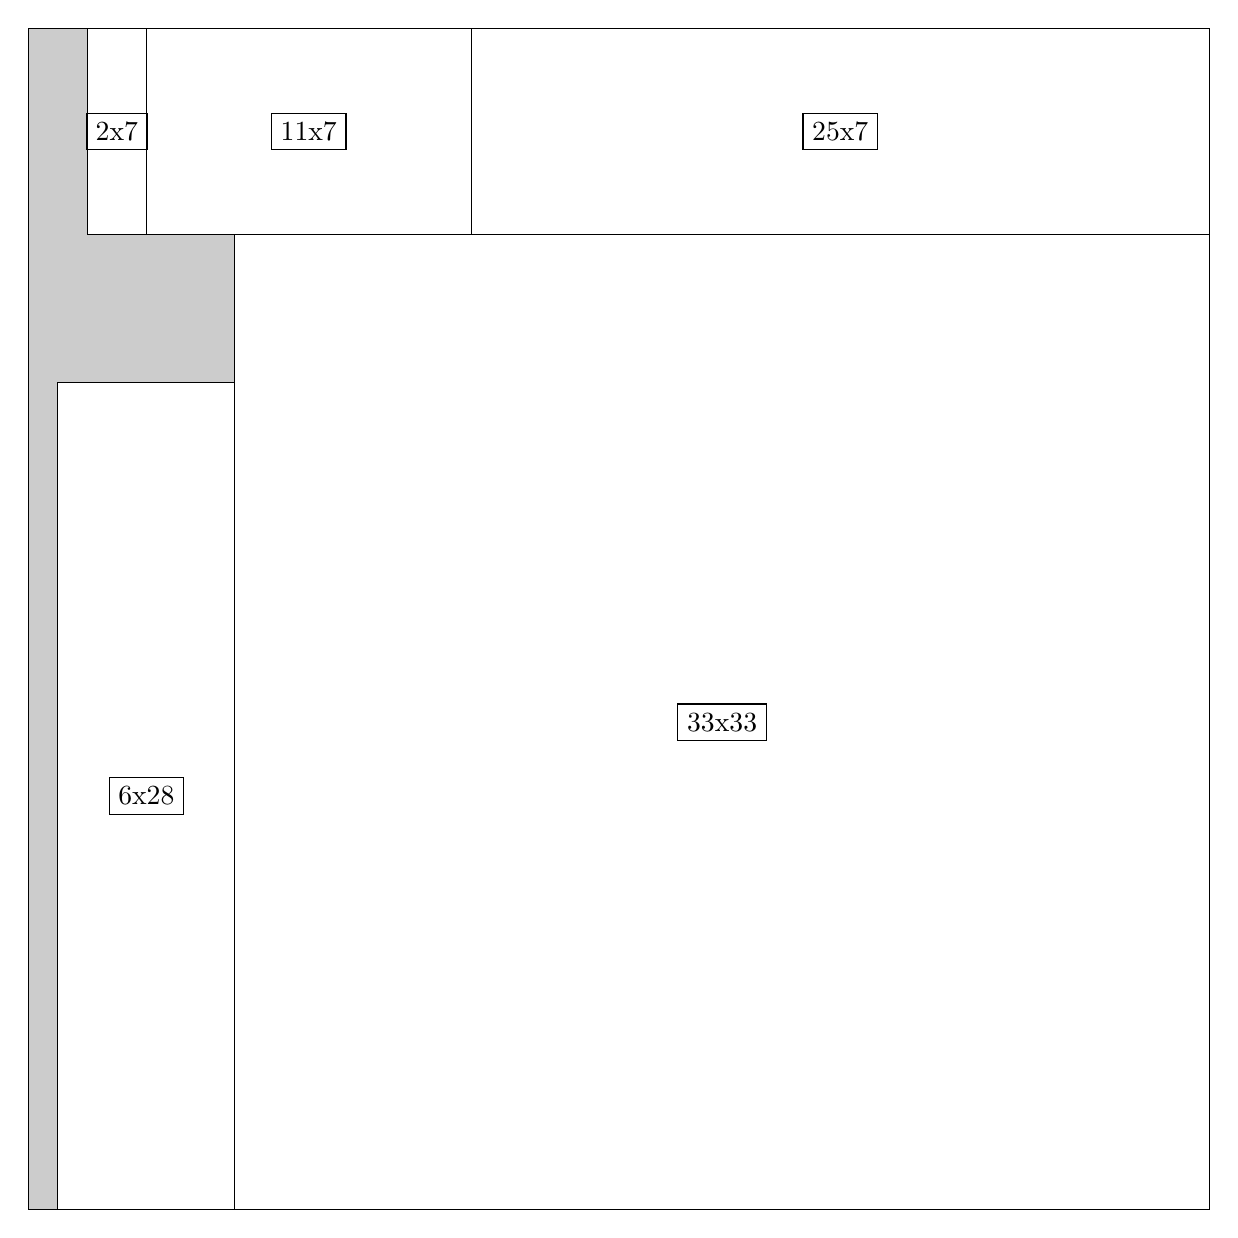
\begin{tikzpicture}[shorten >=1pt,scale=1.0,every node/.style={scale=1.0},->]
\tikzstyle{vertex}=[circle,fill=black!25,minimum size=14pt,inner sep=0pt]
\filldraw[fill=gray!40!white, draw=black] (0,0) rectangle (15.0,15.0);
\foreach \name/\x/\y/\w/\h in {33x33/2.625/0.0/12.375/12.375,6x28/0.375/0.0/2.25/10.5,25x7/5.625/12.375/9.375/2.625,11x7/1.5/12.375/4.125/2.625,2x7/0.75/12.375/0.75/2.625}
\filldraw[fill=white!40!white, draw=black] (\x,\y) rectangle node[draw] (\name) {\name} ++(\w,\h);
\end{tikzpicture}


w =33 , h =33 , x =7 , y =0 , v =1089
\par
w =6 , h =28 , x =1 , y =0 , v =168
\par
w =25 , h =7 , x =15 , y =33 , v =175
\par
w =11 , h =7 , x =4 , y =33 , v =77
\par
w =2 , h =7 , x =2 , y =33 , v =14
\par
\newpage


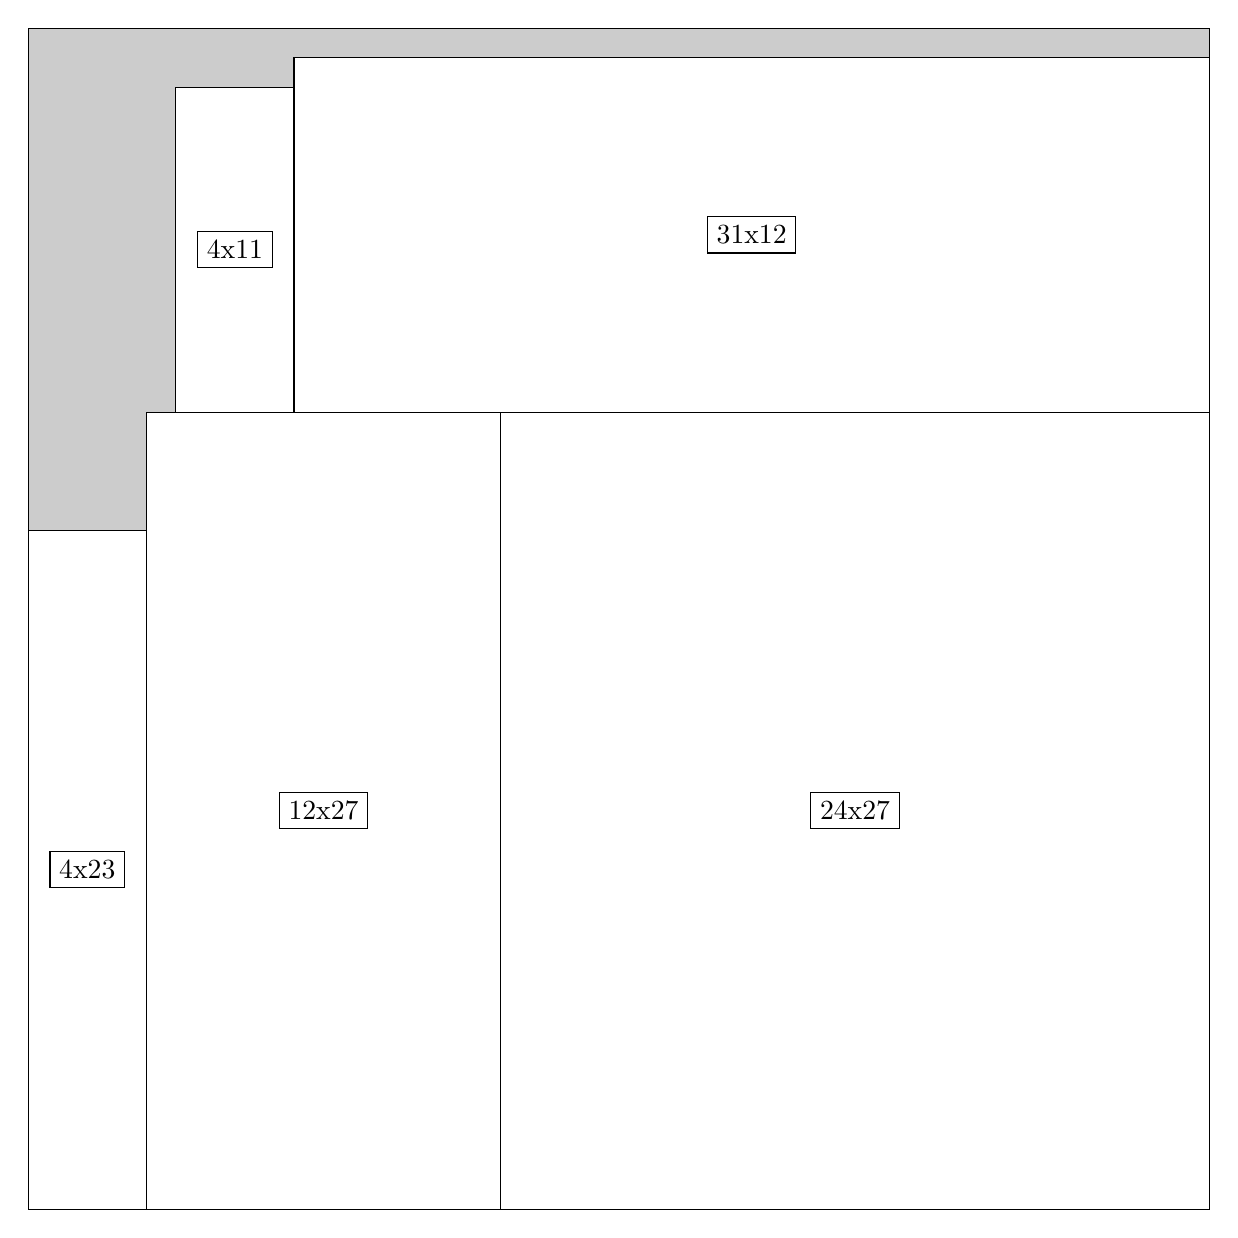
\begin{tikzpicture}[shorten >=1pt,scale=1.0,every node/.style={scale=1.0},->]
\tikzstyle{vertex}=[circle,fill=black!25,minimum size=14pt,inner sep=0pt]
\filldraw[fill=gray!40!white, draw=black] (0,0) rectangle (15.0,15.0);
\foreach \name/\x/\y/\w/\h in {24x27/6.0/0.0/9.0/10.125,12x27/1.5/0.0/4.5/10.125,4x23/0.0/0.0/1.5/8.625,31x12/3.375/10.125/11.625/4.5,4x11/1.875/10.125/1.5/4.125}
\filldraw[fill=white!40!white, draw=black] (\x,\y) rectangle node[draw] (\name) {\name} ++(\w,\h);
\end{tikzpicture}


w =24 , h =27 , x =16 , y =0 , v =648
\par
w =12 , h =27 , x =4 , y =0 , v =324
\par
w =4 , h =23 , x =0 , y =0 , v =92
\par
w =31 , h =12 , x =9 , y =27 , v =372
\par
w =4 , h =11 , x =5 , y =27 , v =44
\par
\newpage


\begin{tikzpicture}[shorten >=1pt,scale=1.0,every node/.style={scale=1.0},->]
\tikzstyle{vertex}=[circle,fill=black!25,minimum size=14pt,inner sep=0pt]
\filldraw[fill=gray!40!white, draw=black] (0,0) rectangle (15.0,15.0);
\foreach \name/\x/\y/\w/\h in {32x21/3.0/0.0/12.0/7.875,32x19/3.0/7.875/12.0/7.125,8x25/0.0/0.0/3.0/9.375,8x15/0.0/9.375/3.0/5.625}
\filldraw[fill=white!40!white, draw=black] (\x,\y) rectangle node[draw] (\name) {\name} ++(\w,\h);
\end{tikzpicture}


w =32 , h =21 , x =8 , y =0 , v =672
\par
w =32 , h =19 , x =8 , y =21 , v =608
\par
w =8 , h =25 , x =0 , y =0 , v =200
\par
w =8 , h =15 , x =0 , y =25 , v =120
\par
\newpage


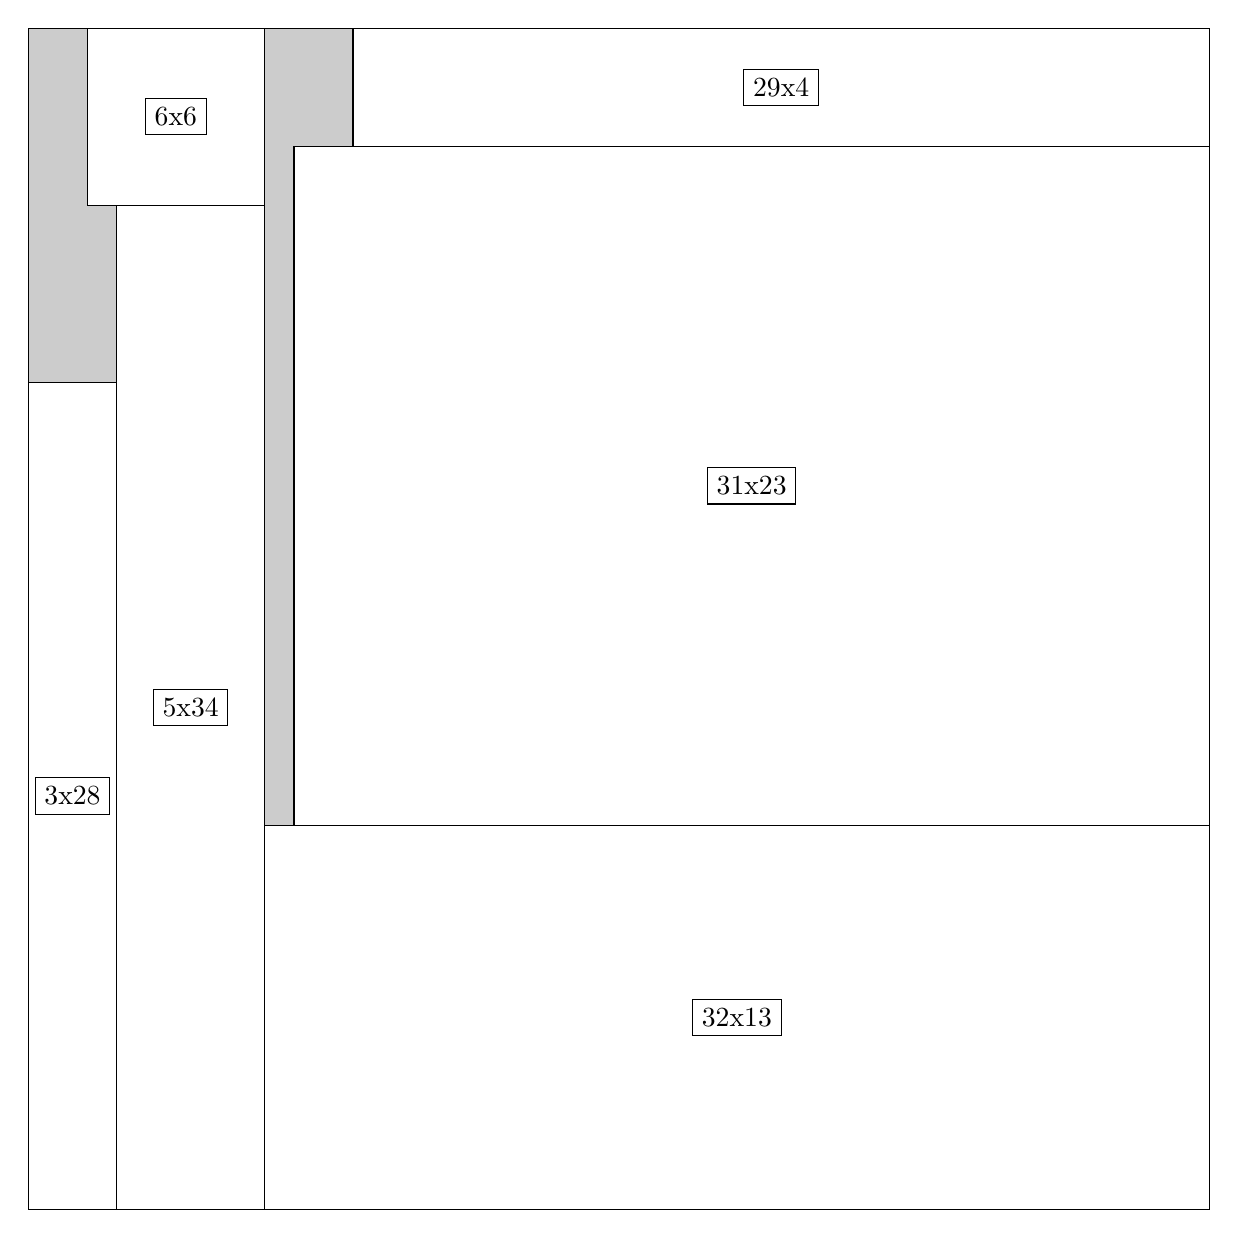
\begin{tikzpicture}[shorten >=1pt,scale=1.0,every node/.style={scale=1.0},->]
\tikzstyle{vertex}=[circle,fill=black!25,minimum size=14pt,inner sep=0pt]
\filldraw[fill=gray!40!white, draw=black] (0,0) rectangle (15.0,15.0);
\foreach \name/\x/\y/\w/\h in {32x13/3.0/0.0/12.0/4.875,31x23/3.375/4.875/11.625/8.625,29x4/4.125/13.5/10.875/1.5,5x34/1.125/0.0/1.875/12.75,3x28/0.0/0.0/1.125/10.5,6x6/0.75/12.75/2.25/2.25}
\filldraw[fill=white!40!white, draw=black] (\x,\y) rectangle node[draw] (\name) {\name} ++(\w,\h);
\end{tikzpicture}


w =32 , h =13 , x =8 , y =0 , v =416
\par
w =31 , h =23 , x =9 , y =13 , v =713
\par
w =29 , h =4 , x =11 , y =36 , v =116
\par
w =5 , h =34 , x =3 , y =0 , v =170
\par
w =3 , h =28 , x =0 , y =0 , v =84
\par
w =6 , h =6 , x =2 , y =34 , v =36
\par
\newpage


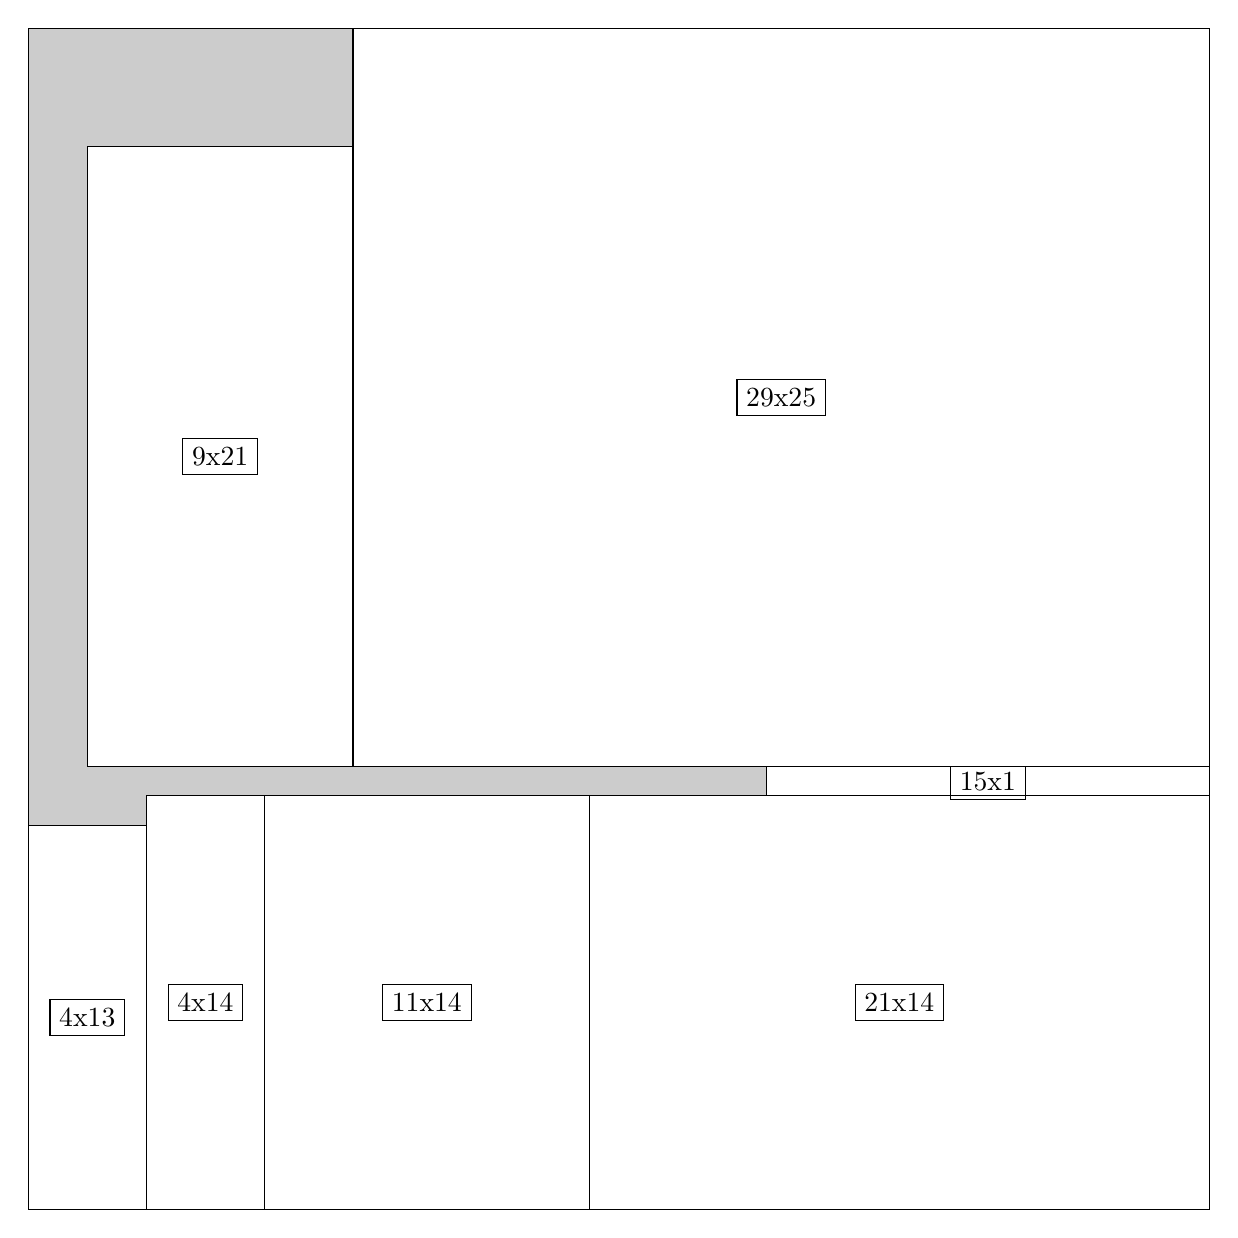
\begin{tikzpicture}[shorten >=1pt,scale=1.0,every node/.style={scale=1.0},->]
\tikzstyle{vertex}=[circle,fill=black!25,minimum size=14pt,inner sep=0pt]
\filldraw[fill=gray!40!white, draw=black] (0,0) rectangle (15.0,15.0);
\foreach \name/\x/\y/\w/\h in {21x14/7.125/0.0/7.875/5.25,15x1/9.375/5.25/5.625/0.375,11x14/3.0/0.0/4.125/5.25,4x14/1.5/0.0/1.5/5.25,4x13/0.0/0.0/1.5/4.875,29x25/4.125/5.625/10.875/9.375,9x21/0.75/5.625/3.375/7.875}
\filldraw[fill=white!40!white, draw=black] (\x,\y) rectangle node[draw] (\name) {\name} ++(\w,\h);
\end{tikzpicture}


w =21 , h =14 , x =19 , y =0 , v =294
\par
w =15 , h =1 , x =25 , y =14 , v =15
\par
w =11 , h =14 , x =8 , y =0 , v =154
\par
w =4 , h =14 , x =4 , y =0 , v =56
\par
w =4 , h =13 , x =0 , y =0 , v =52
\par
w =29 , h =25 , x =11 , y =15 , v =725
\par
w =9 , h =21 , x =2 , y =15 , v =189
\par
\newpage


\end{document}